\section{In-medium SRG: Wegner's generator}
\label{sec:IMSRGres}
Now that we have verified that the SRG evolution yields the correct result in free space, we will perform the runs in medium. We will especially focus on how the truncation error effects the results. Since the in-medium approach allows us to study systems with a much higher number of basis states, we will study how the ground state energy $E_0$ behaves as the number of particles $N$ and shells $R$ is increased. Unless otherwise stated, all runs until section \ref{sec:White} are performed with Wegner's canonical generator $\hat{\eta}_s = \left[ \Hd_s, \Ho_s \right]$.

\subsection{Code validation}
As we did for the free-space approach, it is important to check that the code gives reliable results and is free of bugs. An important benchmark is the free-space evolution, which does not contain any truncation errors. Since a system with $N=2$ particles can maximally have two-particle-two-hole excitations, we know that IM-SRG(2) should be exact as long as we also include the loop terms of higher-order interactions. With those loop terms we mean effective two-body terms of the form
\[
\langle p q || r s \rangle = \sum_i \langle p q i | v^{(3)} | r s i \rangle,
\]
and effective one-body terms of the form
\[
f_{pq} = \frac{1}{2}\sum_{ij} \langle p i j | v^{(3)} | q i j \rangle, 
\] 
where $i$ and $j$ sums over all hole states. We want to remind the reader that in our model of quantum dots, three-body interactions are not present from the beginning on. Instead, they are generated during the flow and higher order-correlations evolve first in the generator $\hat{\eta}$ and are then transferred to the Hamiltonian by $\frac{d \hat{H}_s}{ds} = \left[ \hat{\eta}_s, \hat{H}_s \right]$. \\
If we want to exclude truncation errors for two particles, we therefore need to consider those effective one- and two-body terms for the generator $\hat{\eta}$ as well as for the interaction terms of the Hamiltonian.


\begin{table}
\begin{center}
\begin{tabular}{cccc}
\hline\hline
$\omega$ & $R$ & In-medium SRG& Free space SRG \\
\hline
0.1 & 3 & 0.4421887603&0.4421887603  \\
& 5 &  0.4416137068& 0.4416137068\\
& 7 &0.4413297357 & 0.4413297357\\
\hline
0.28 & 3 &1.032681412 &1.032681412 \\
& 5 &1.026588059 & 1.026588059\\
& 7 & 1.024705875 & 1.024705875 \\
\hline
0.5 & 3 &1.681631996 &1.681631996 \\
& 5 &1.669498218 &1.669498218 \\
& 7 &1.665799351 &1.665799351 \\
\hline
1.0 & 3 &3.038604576 &3.038604576 \\
& 5 & 3.017606230& 3.017606230\\
& 7 & 3.011019984& 3.011019984\\
\hline\hline
\end{tabular}
\caption{Comparison of the ground state energy $E_0$ in free space and IM-SRG(2/3) for $N=2$ particles. With IM-SRG(2/3) we denote second-order IM-SRG(2), extended by the loop terms of three-body interactions. The high number of specified digits shall emphasize that exactly the same result is obtained. 
All runs are performed with HO basis and standard interaction.}
\label{tab:CompIMFree}
\end{center}
\end{table}

Table \ref{tab:CompIMFree} shows that we obtain exactly the same results as in free space. First, this implies that the flow equations are correctly implemented. Second, we see that as long as the result is converging, the in-medium approach does not introduce greater numerical roundoff errors etc., which would give a deviating result. Dealing with numerical methods, one should always check this since there exist many methods that are theoretically exact, but still give unstable results due to numerical issues.

\subsection{Numerical results with IM-SRG(2)}

Having verified that the flow equations are correctly implemented, we will first start with $N=2$ particles. This will enable us to make statements about how the truncation error affects the results, since we have the possibility to compare with the IM-SRG(2/3) approach that also includes the loop terms of three-body interactions.

\begin{table}
\begin{center}
\begin{tabular}{cccc}
\hline\hline
 $R$ & IM-SRG(2)& IM-SRG(2/3)& Rel.Diff. \\
\hline
 3 & 3.033884 &3.038605 & 0.16\%\\
 4 & 3.018303 &3.025231 & 0.23\%\\
5 &  3.012019 &3.017606 & 0.19\%\\
6 &  3.008581 &3.013626 & 0.17\%\\
7 &  3.006509& 3.011020 & 0.15\%\\
8 &  3.005058& 3.009236 & 0.14\%\\
9 &  3.004008& 3.007929 & 0.13\%\\
10 & 3.003198& 3.006937 & 0.12\%  \\
\hline
\end{tabular}
\caption{Comparison of the ground state energy $E_0$ obtained with IM-SRG(2) and \mbox{IM-SRG(2/3)}, which is expanded by the loop terms of three-body interactions. We performed the runs for $N=2$ particles, an oscillator frequency $\omega=1.0$, standard interaction and  HO basis. The ground state energy is given in units of $\left[ E_H \right]$. The last column lists the relative error $\left|E_{0[\text{IM-SRG}(2/3)]}-E_{0[\text{IM-SRG}(2)]}\right|/E_{0[\text{IM-SRG}(2/3)]}$.}
\label{tab:CompIM23}
\end{center}
\end{table}

\begin{figure}
\begin{center}
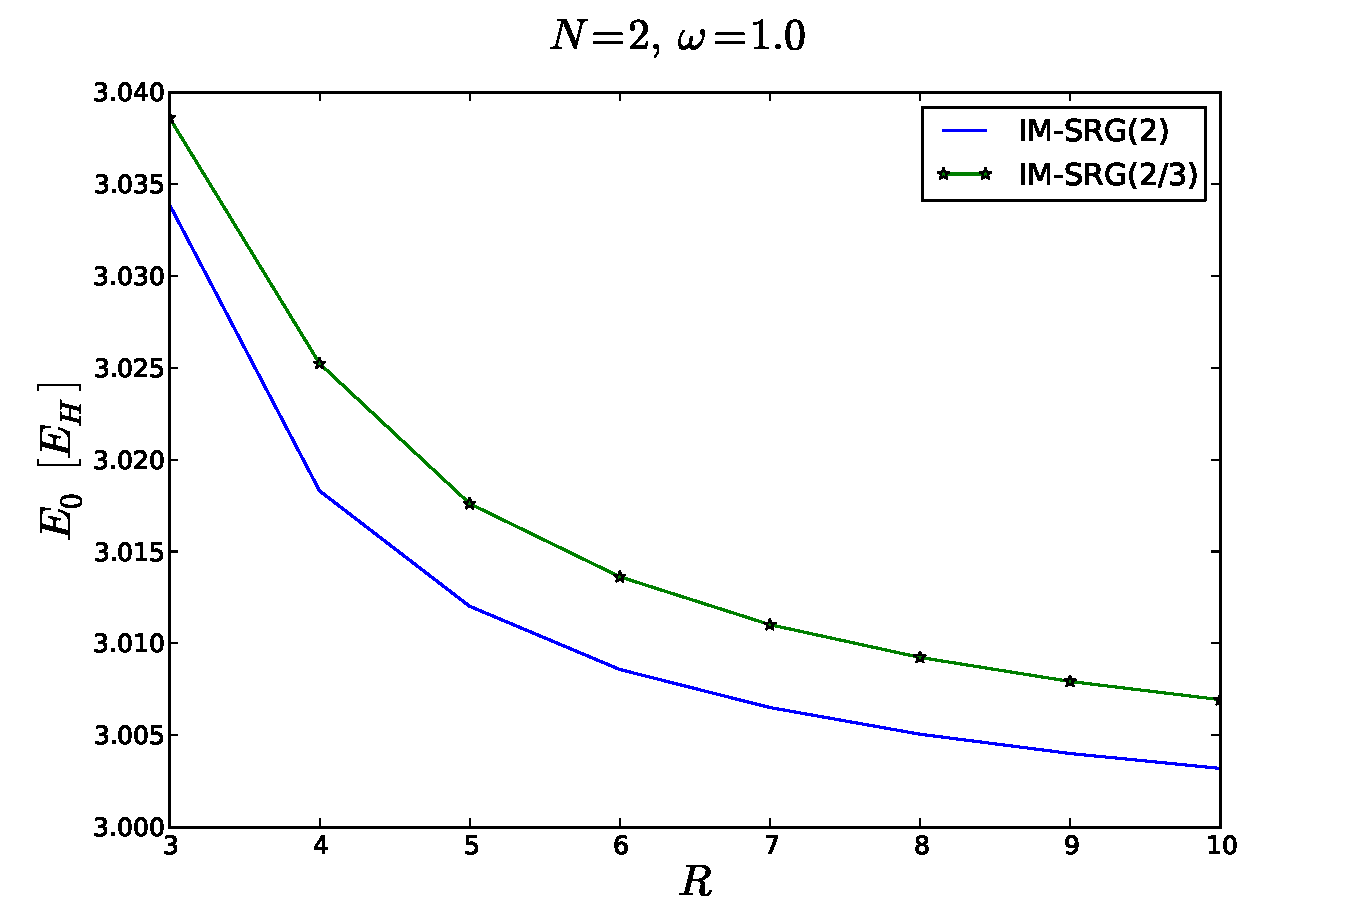
\includegraphics[scale=0.4]{../Plots/imsrg23.pdf}
\end{center}
\caption{Ground state energy $E_0$ for $N=2$ particles as function of the shell number $R$. The result obtained with IM-SRG(2) is compared with the one of IM-SRG(2/3), which also contains the loop terms of three-body interactions. All runs have been performed with oscillator frequency $\omega = 1.0$, HO basis and standard interaction.}
\label{fig:imsrg23}
\end{figure}

From table \ref{tab:CompIM23} and figure \ref{fig:imsrg23} we conclude that the truncation error generally results in a lower ground state energy $E_0$ than the untruncated result. The relative error lies mainly between $0.1 \%$ and $0.2 \%$ and seems to diminish slightly as the number of shells $R$ is increased. Since a larger number of basis states takes care of higher order correlations, we are more interested in those results, anyway, and the trend of a smaller relative error is a desirable feature.

Before we move on to more results, it seems necessary to explain why we have chosen not to include the three-body terms in our further calculations. The advantage would be to introduce a smaller truncation error in the flow equations, but the computational cost would be much higher. Instead of Eqs. (\ref{eq:flow2order1})-(\ref{eq:flow2order}), we would have to solve Eqs. (\ref{eq:flow0})-(\ref{eq:flow3}) each time the derivative function is called by the ODE solver. This would involve a considerably larger number of terms, with the maximal number of indices to be summed over increased from four to six. However, even with IM-SRG(3) we would still have a truncation error for systems with $N=6,12,\dots$ particles.
 This means that the huge number of additional terms due to three-body interactions would just improve, but not eliminate the truncation error. It therefore remains a question of how much additional CPU time one is willing to spend for a slight improvement of the result. In this thesis, we have decided to restrict us to IM-SRG(2) and rather focus on how to improve convergence within the limitations of this approach.

\subsection{Convergence analysis}

Analogously to the free-space case, we first look at the easiest example of $N=2$ particles with standard Coulomb interaction and harmonic oscillator basis. 
That way, we can identify 
%abnormalities in the convergence pattern and 
potential problems of the SRG method, before we move on to higher number of particles and methods to improve convergence.

\begin{table}
\begin{center}
\begin{tabular}{cccccc}
\hline\hline
$R$  & $\omega = 0.1$ & $\omega = 0.28$ & $\omega=0.5$ & $\omega=1.0$ \\
\hline
2  &nc & 1.089121&1.767956 &3.143526 \\
3  &0.4252721 &1.022391 &1.674052 &3.033884 \\
4  &0.4254326 &1.014839 &1.663100 &3.018304 \\
5  &0.4284273 &1.016052 &1.661176 &3.012019 \\
6  &0.4354808 &1.017138 &1.660178 & 3.008581\\
7  &0.4368345 &1.017620 &1.659615 &  3.006510\\
8  &0.4367619 &1.017846 &1.659181 & 3.005059\\
9  &0.4368605 &1.017956 &1.658851 &3.004009 \\
10 &0.4371156 &1.018009 &1.658578 &3.003198 \\
11 &0.4371817 &1.018017 &1.658347 &3.002555 \\
12 &0.4372050 &1.018006 &1.658150 &3.002031 \\
\hline
DMC &0.44087(3) &1.02166(3) &1.65975(2) &3.00000(3) \\ % redo: 0.5,0.1
\hline\hline
\end{tabular}
\end{center}
\caption{Ground state energy $E_0$ (in $\left[E_H\right]$) for a system with $N=2$ particles, HO basis and standard Coulomb interaction. For benchmarking, the last line shows the corresponding result that we got with Diffusion Monte Carlo (DMC). The convergence behaviour is illustrated in figure \ref{fig:convergence00}.}
\label{tab:imsrg2-2part}
\end{table}

\begin{figure}
\begin{center}
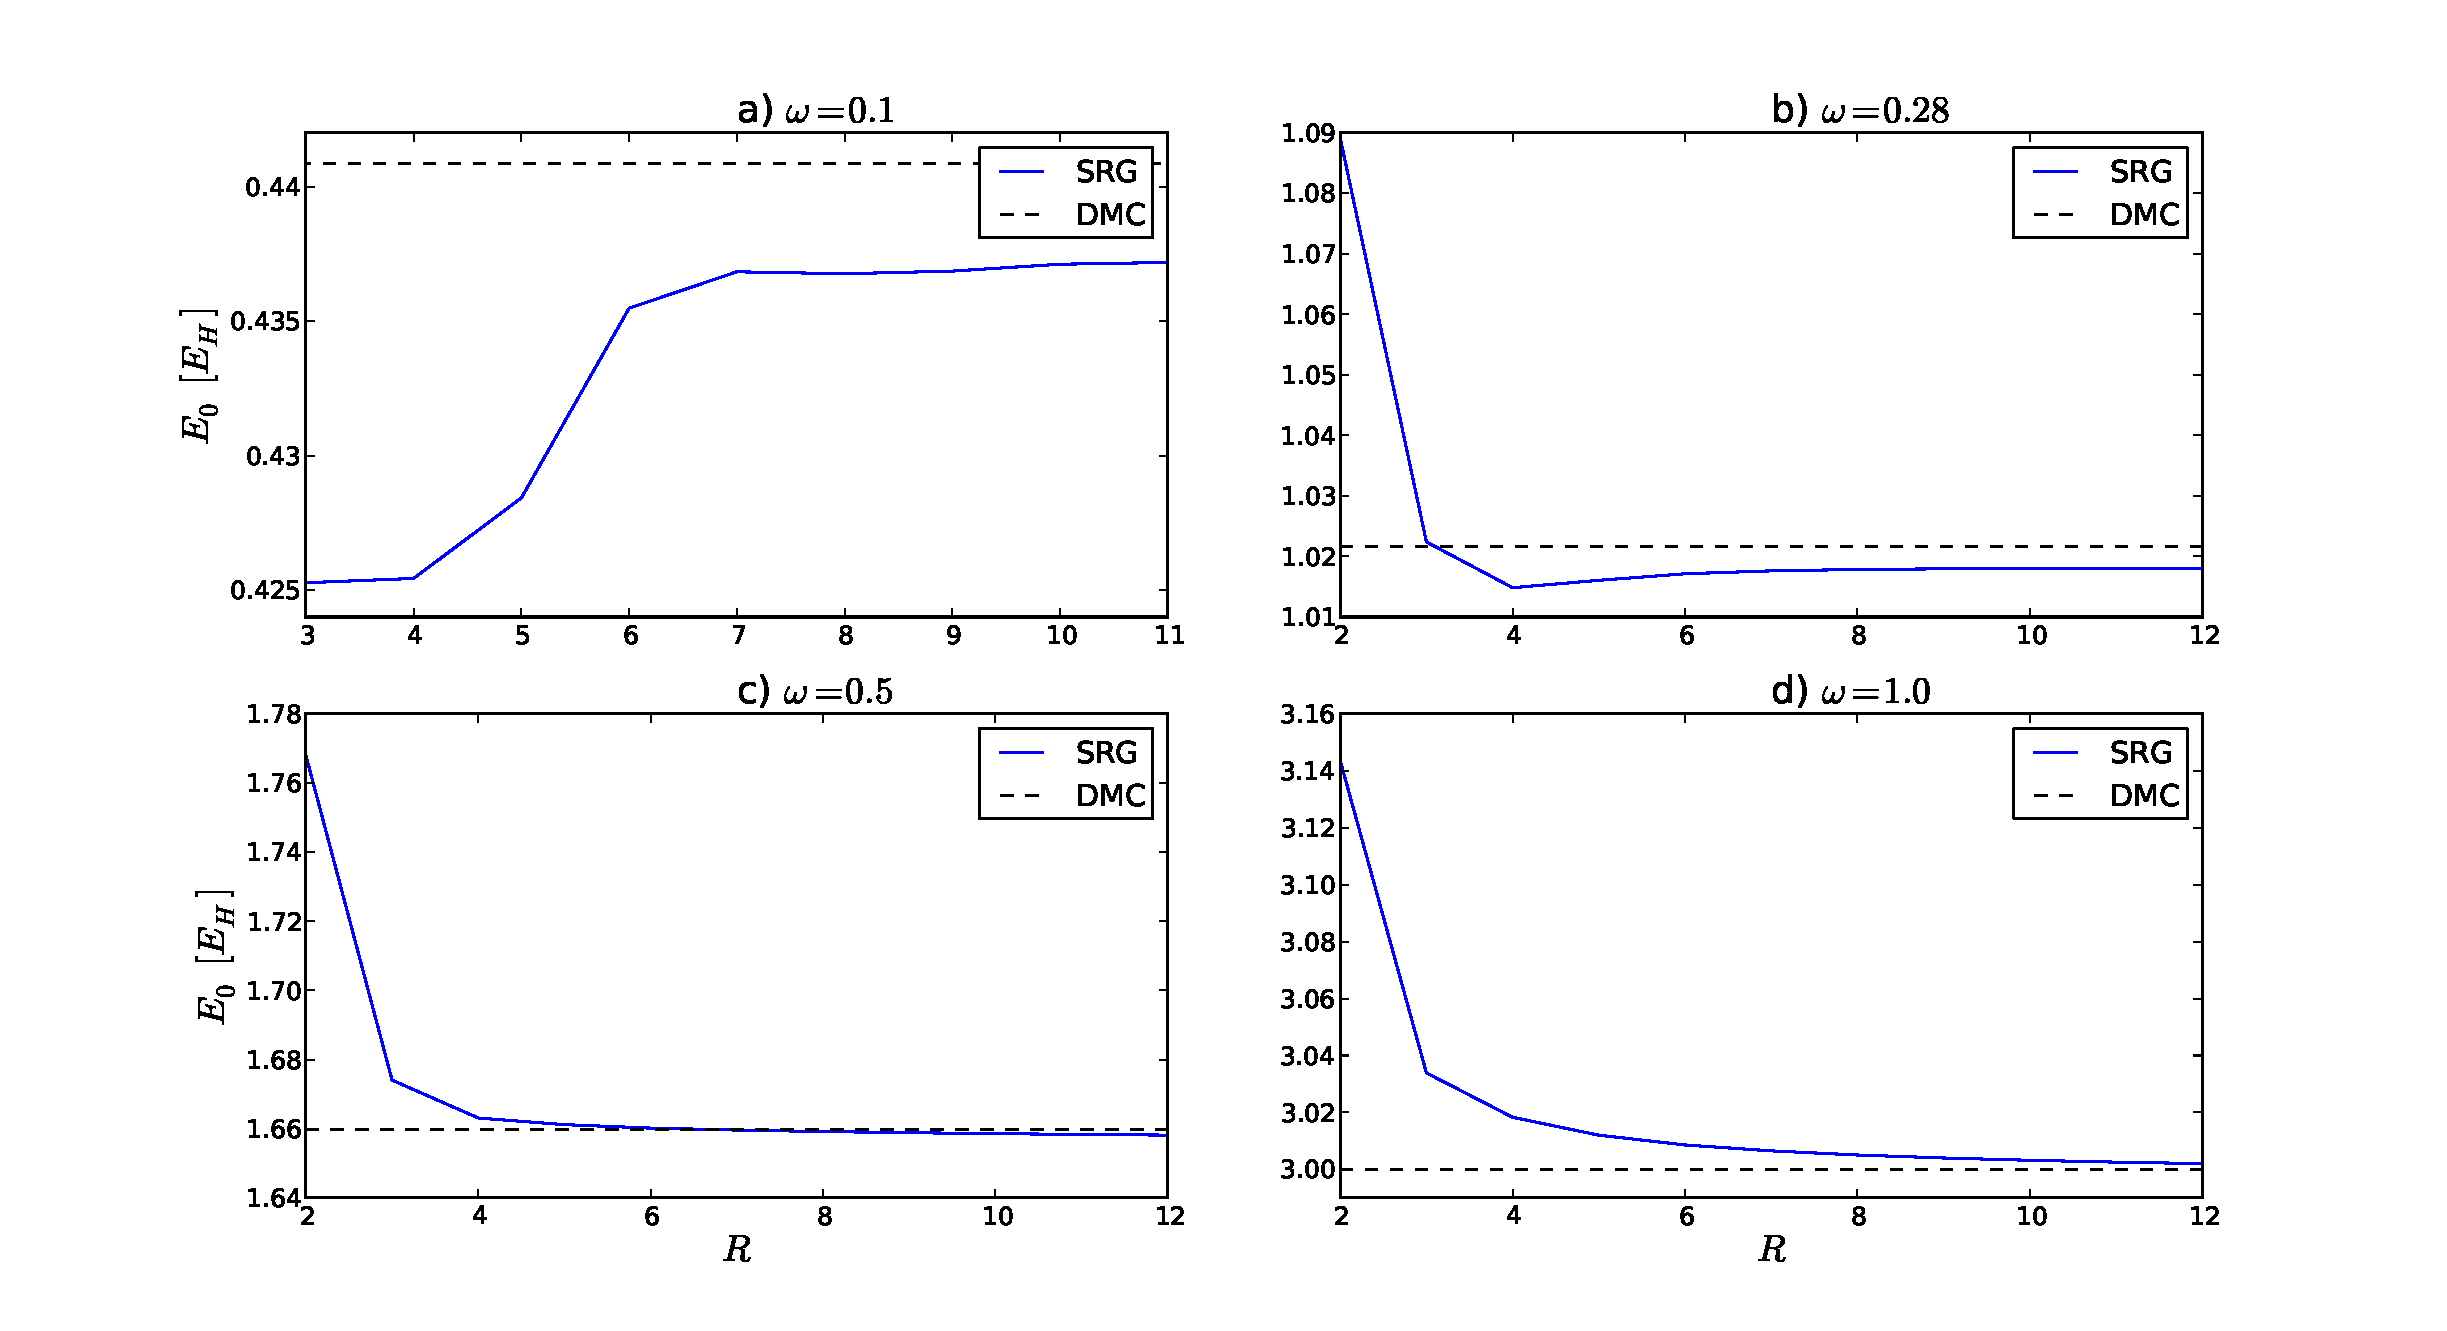
\includegraphics[scale=0.4]{../Plots/convergence00.pdf}
\end{center}
\caption{Convergence behaviour of the ground state energy $E_0$ as function of the shell number $R$. All runs have been performed with $N=2$ particles, HO basis and standard Coulomb interaction. The SRG results are compared with the ones obtained from Diffusion Monte Carlo (DMC) caculations.}
\label{fig:convergence00}
\end{figure}

Table \ref{tab:imsrg2-2part} and figure \ref{fig:convergence00} present the obtained results as function of the shell number $R$. Since we are especially interested in whether an increase of $R$ causes $E_0$ to converge to the exact result, we also
performed Diffusion Monte Carlo (DMC) calculations for benchmarking. 

The first observation is that the convergence behaviour is qualitatively different, depending on the oscillator frequency $\omega$. For $\omega=0.1$ and $\omega=0.28$, the energy seems to be converging towards the DMC result  from below, whereas for $\omega=1.0$, convergence takes place from above. For $\omega=0.5$, $E_0$ is decreasing as function $R$ and it first appears as if the DMC result is reached from above. However, the ground state energy does not stop at the DMC value, but is further decreasing and getting too low. Since a larger number of shells $R$ means that also higher-order correlations are taken into account, we actually hope for convergence towards the analytically correct result for $R\rightarrow\infty$. In plot $c)$ with $\omega=0.5$, this is definitely not reached and a similar trend seems possible for $\omega=1.0$.\\
Since for $N=2$ particles, the SRG method involves the smallest truncation error, we do not expect better results for $N=6$ particles and will therefore try to improve convergence by an effective interaction and a Hartree-Fock basis, before we move on to more particles.

\subsection{Improving convergence: Effective interaction and Hartree-Fock basis}
\label{subsec:WegnerEffHF}

\subsubsection{Effective interaction}
As explained in section \ref{subsec:FreeEffAndHF}, effective interactions can be used to speed up  convergence as function of the shell number $R$. For our SRG calculations in medium, we use the same effective interaction as we did in free space, namely a unitary transformation of the two-body Hamiltonian, implemented in the OpenFCI library \cite{Kvaalcode}. As explained before, this should yield the exact ground state energy $E_0$ for  $N=2$ particles when the Hamiltonian is diagonalized and this result should be independent of the number of shells $R$. For a larger number of particles $N$, the result will no longer be exact, but we still expect it to be a better approximation than a standard Coulomb interaction. \\
Moreover, in analogy to the free-space case, we will use the effective interaction without energy cut. This introduces a small additional error but makes the SRG runs numerically much more stable, especially as the oscillator frequency $\omega$ is lowered.

\begin{figure}
\begin{center}
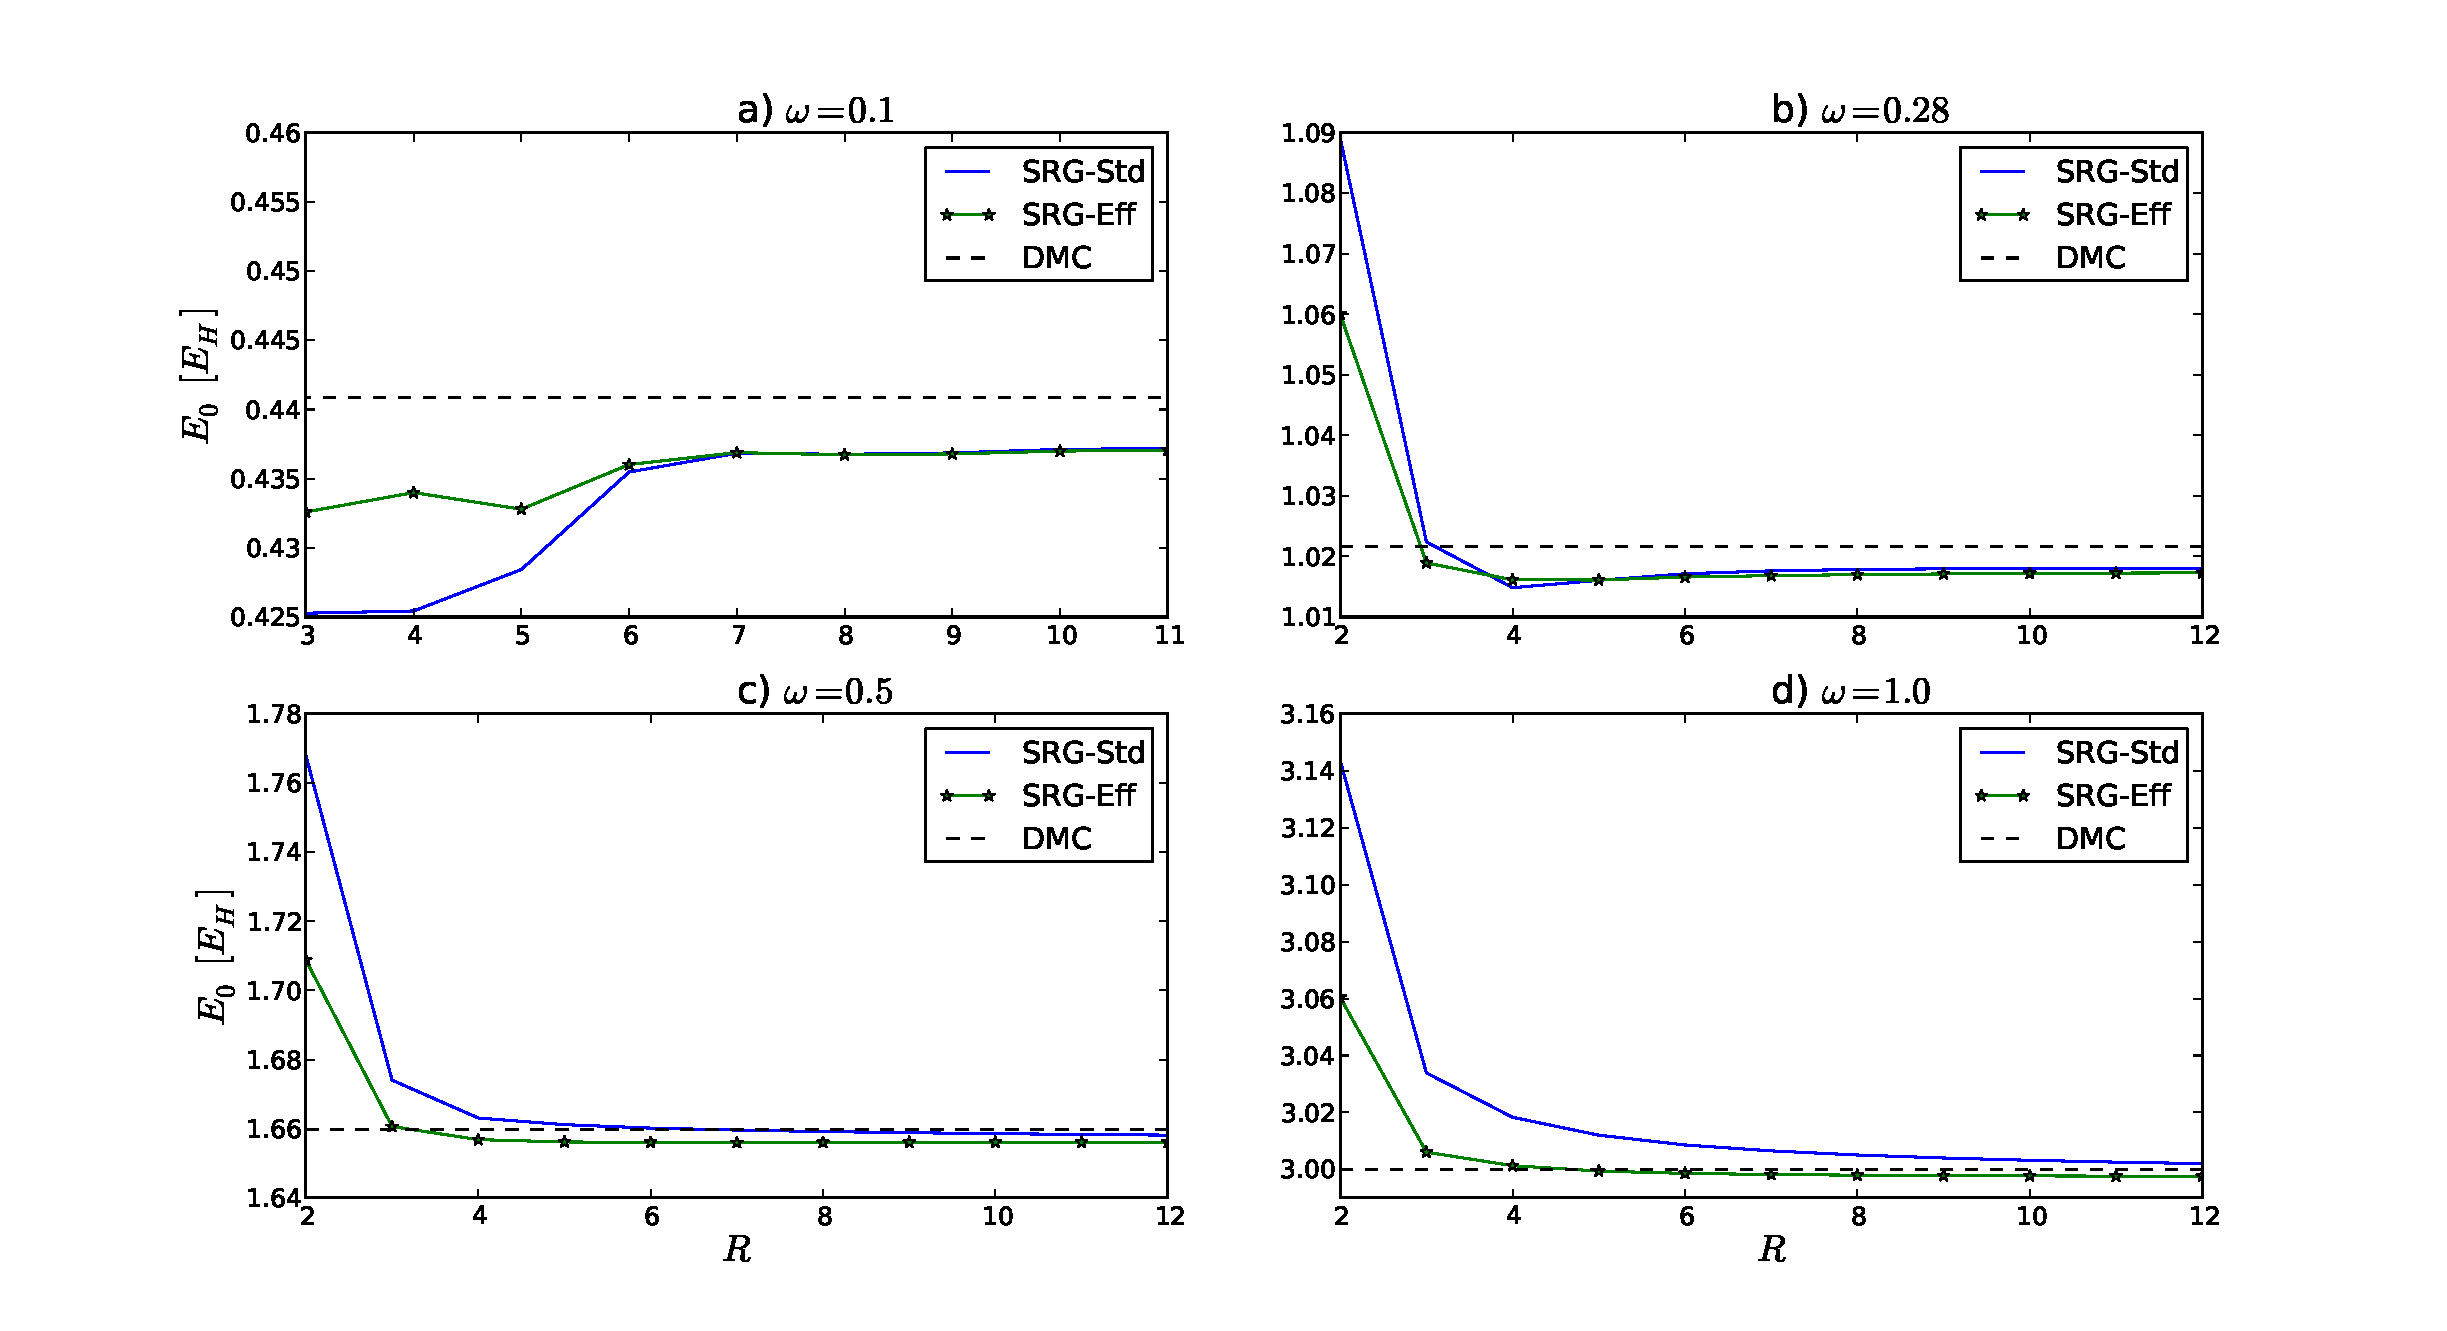
\includegraphics[scale=0.4]{../Plots/convergence01.pdf}
\end{center}
\caption{Comparison of the ground state energy $E_0$ between SRG with standard Coulomb interaction (SRG-Std) and effective interaction (SRG-Eff). All runs have been performed with $N=2$ particles and HO basis. For benchmarking, the plots also include the corresponding DMC result.}
\label{fig:convergence01}
\end{figure}

\begin{table}
\begin{center}
\begin{tabular}{cccccc}
\hline\hline
$R$  & $\omega = 0.1$ & $\omega = 0.28$ & $\omega=0.5$ & $\omega=1.0$ \\
\hline
2  &0.4552503 &1.060039 &1.708803 &3.060394 \\
3  &0.4325924 &1.018938 &1.660647 &3.006047 \\
4  &0.4339930 &1.016126 &1.656843 &3.001313 \\
5  &0.4327919 &1.016113 &1.656178 &2.999413 \\
6  &0.4360176 &1.016597 &1.656036 &2.998598 \\
7  &0.4368824 &1.016830 &1.656023 &2.998209 \\
8  &0.4367201 &1.016996 &1.656036 &2.997970 \\
9  &0.4367887 &1.017110 & 1.656056 &2.997824 \\
10 &0.4369907 &1.017197 &1.656072 &2.997719 \\
11 &0.4370701 &1.017252 &1.656082 &2.997641 \\
12 &0.43711739 &1.017292 &1.656087 &2.997581 \\
\hline
DMC &0.44087(3) &1.02166(3) &1.65975(2) &3.00000(3) \\ % redo: 0.5,0.1
\hline\hline
\end{tabular}
\end{center}
\caption{Ground state energy $E_0$ (in $\left[E_H\right]$) for a system with $N=2$ particles, HO basis and effective interaction. For benchmarking, we also give the results that we got with Diffusion Monte Carlo (DMC). 
 }
\label{tab:imsrg2-2parteff}
\end{table}

In order to make statements about how the results are affected, we performed the same runs as in table \ref{tab:imsrg2-2part}, this time using an effective interaction. The numerical results can be found in table \ref{tab:imsrg2-2parteff}. Figure \ref{fig:convergence01} compares directly the runs with effective interaction with the previous ones using a standard Coulomb interaction.\\
The major observation is that generally, the effective interaction does not yield a better result. Except for $\omega=0.1$, the obtained ground state energy is lower than with standard interaction, which makes the already too small results (with respect to the DMC calculations) even slightly worse.\\
We also performed calculations with $N=6$ particles, where the truncation error made by IM-SRG(2) is larger. As shown in table \ref{tab:imsrg2-6parteff}, the ground state energy $E_0$ gets again too low as the number of shells $R$ is increased. Additionally, for low values of the oscillator frequency $\omega$, our results are not converging. This observation is analogous to the free-space case and we suspect numerical instabilities in the ODE solver to be responsible for this effect. Since a lower oscillator frequency corresponds to higher correlations between the particles, it seems that our method gets unstable as the correlations are increased. This behaviour has also been observed for other ab-initio many-body methods, e.g. by previous master students studying circular quantum dots with the Coupled Cluster method \cite{Christoffer,Lohne}.\\
The unsuitable results as the number of shells $R$ is increased, as well as non-convergence for lower values of $\omega$, motivate to exchange the harmonic oscillator by a Hartree-Fock basis and study the convergence behaviour using this basis.


\begin{table}
\begin{center}
\begin{tabular}{cccccc}
\hline\hline
$R$  & $\omega = 0.1$ & $\omega = 0.28$ & $\omega=0.5$ & $\omega=1.0$ \\
\hline
3 & nc&nc &12.36436 & 20.85382 \\
4 & nc&7.69353 &11.85851&20.20328 \\
5 & nc&7.63149 &11.81564&20.18527 \\
6 &nc &7.54028 &11.77229 & 20.16104 \\
7 &nc & nc & 11.76773 & 20.15487 \\
8 &nc & nc & 11.76193 & 20.15073  \\
9 &nc  & nc  & 11.76187 & 20.14857 \\
10 &nc & nc&11.76192 & 20.14719 \\
\hline
DMC& - & 7.6001(2)&11.7888(2) &20.1598(4) \\ %REDO: 0.1,0.5
\hline\hline
\end{tabular}
\end{center}
\caption{Ground state energy $E_0$ (in $\left[E_H\right]$) for a system with $N=6$ particles, HO basis and effective interaction. The label ''nc'' denotes non-converging runs.}
\label{tab:imsrg2-6parteff}
\end{table}

\subsubsection{Hartree-Fock basis}

Introducing a Hartree-Fock (HF) basis, the elements corresponding to one-particle-one-hole excitations are already zeroed out when the Hamiltonian in this basis is set up. That way, $\hat{H}$ is already more diagonal from the beginning on, which facilitates the work required of the SRG method. Especially for Wegner's generator, this approach is expected to be very helpful, since the one-body-one-hole excitations link states with comparably low energy difference. Therefore those elements are usually the last ones to be zeroed out and might result in a stiff system of differential equations, requiring many integration steps. Initially giving no contribution with a HF basis, we therefore hope for a faster convergence of our SRG results.\\
Moreover, the Hartree-Fock calculation does not introduce a truncation error like the SRG method does, that is, starting with a Hartree-Fock basis, exact diagonalization yields the same result as with a harmonic oscillator basis. The Hartree-Fock calculation can thus be regarded as first step of diagonalization, but without the truncation error of the SRG method. For this reason, we expect the results to be closer to the exact ones.

\begin{table}
\begin{center}
\tabcolsep=0.07cm
\begin{tabular}{|c|cccc|cccc|}
\hline\hline
& \multicolumn{4}{c}{Standard} & \multicolumn{4}{c|}{Effective} \\
$R$  & $\omega = 0.1$ & $\omega = 0.28$ & $\omega=0.5$ & $\omega=1.0$ & $\omega = 0.1$ & $\omega = 0.28$ & $\omega=0.5$ & $\omega=1.0$\\
\hline
2 &nc &1.089121 &1.767956 & 3.143526 & 0.4552503&1.060039 &1.708804 &3.060394 \\
3 & 0.4354154&1.027421 &1.677713 & 3.036218 &0.4360931 &1.020688 &1.662112 & 3.007167\\
4 & 0.4267331&1.018093 &1.665905 & 3.020183  &0.4330903 &1.017199 &1.658105 &3.002366 \\
5 &0.4362793 &1.020519 & 1.664304& 3.013951 &0.4363536 &1.018151 &1.657803 &3.000586 \\
6 &0.4371191 &1.020532&1.662897 &3.010398  &0.4369135 &1.018444 &1.657671 &2.999826 \\
7 &0.4382300 &1.020842 &1.662244 & 3.008294 &0.4376575 &1.018825 &1.657765 &2.999499 \\
8 &0.4384303 &1.020830 &1.661674 & 3.006790 &0.4379233 &1.019021 &1.657810 &2.999289 \\
9 &0.4385010 &1.020767 &1.661239 & 3.005695 &0.4380649 &1.019142 &1.657844 & 2.999158 \\
10 &0.4385023 &1.020669 &1.660874 & 3.004841  &0.4381416 &1.019214 &1.657860 &2.999059 \\
11 &0.4384803 &1.020565 &1.660568 & 3.004162 &0.4381797 &1.019255 &1.657864 &2.998982 \\
12 &0.4384559 & 1.020467&1.660310 & 3.003607 &0.4382028 &1.019280 &1.657862 & 2.998920\\
\hline
DMC &0.44087(3) &1.02166(3) &1.65975(2) &3.00000(3) & 0.44087(3) &1.02166(3) &1.65975(2) &3.00000(3)\\ % redo: 0.5,0.1
\hline\hline
\end{tabular}
\end{center}
\caption{Ground state energy $E_0$ (in $\left[E_H\right]$) for a system with $N=2$ particles and HF basis. For benchmarking, the last line shows the corresponding result that we got with Diffusion Monte Carlo (DMC). The comparison with HO basis is illustrated in figure \ref{fig:convergence1}. }
\label{tab:imsrg2-2partho}
\end{table}

\begin{figure}
\begin{center}
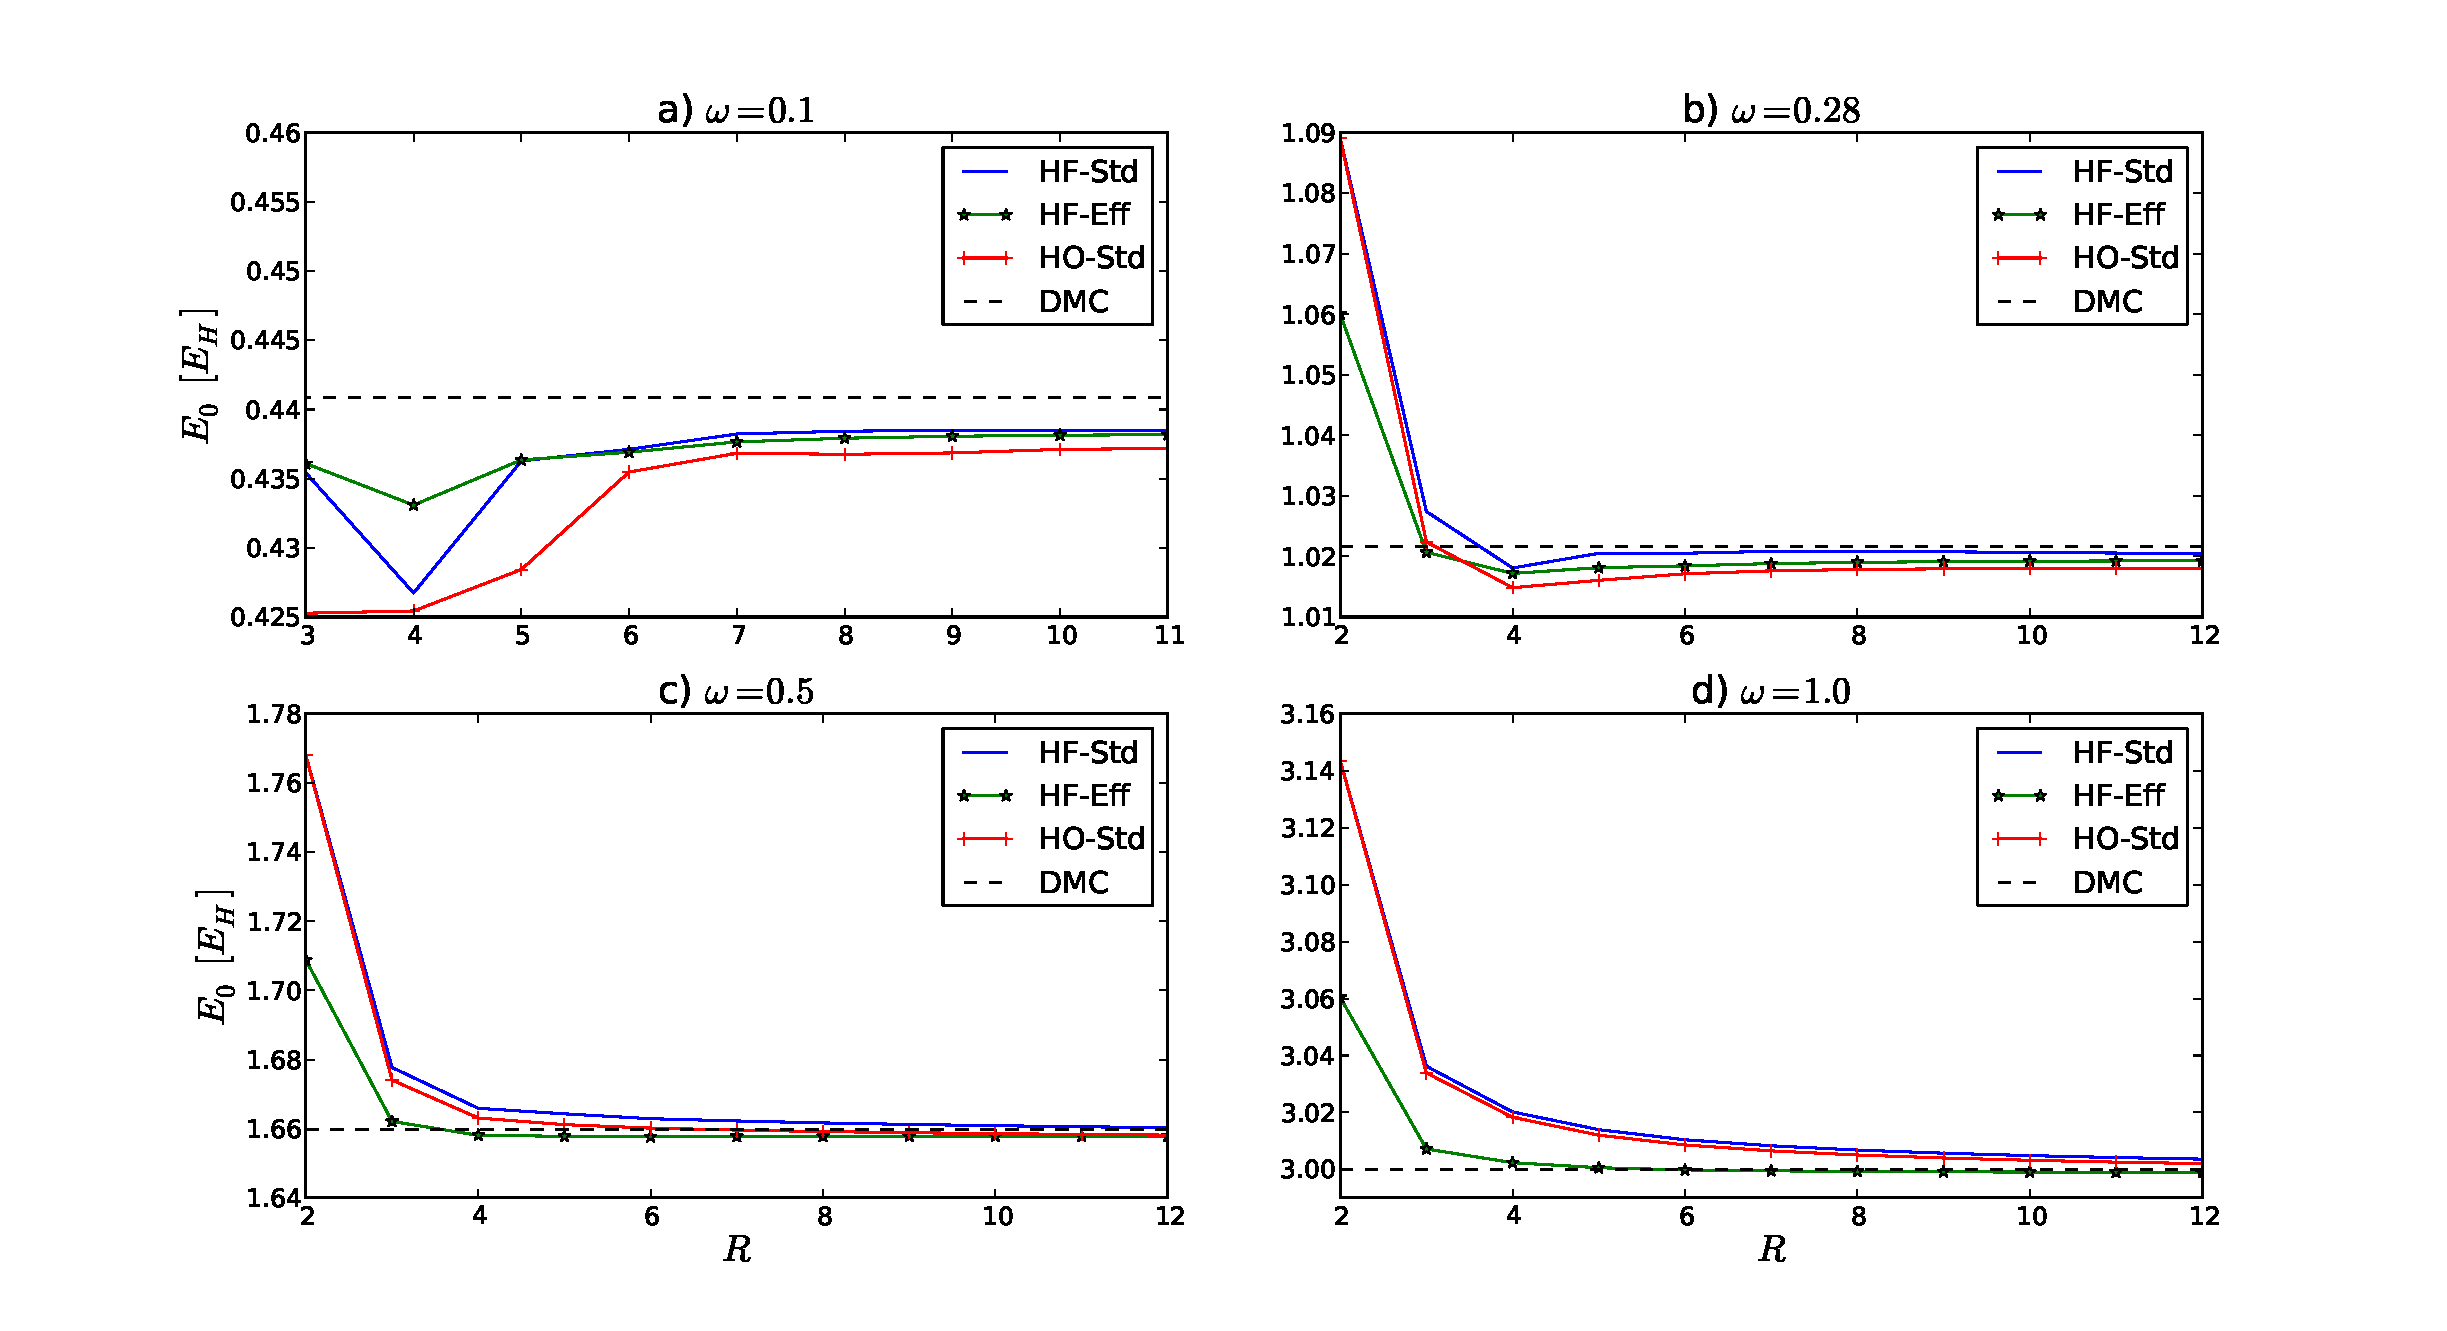
\includegraphics[scale=0.42]{../Plots/convergence1.pdf}
\end{center}
\caption{Comparison between the results with harmonic oscillator (HO) basis and Hartree-Fock (HF) basis. All runs have been performed with $N=2$ particles. For the HO basis, the plots show the result with standard interaction (HO-Std); for the HF basis, both standard interaction (HF-Std) and effective interaction (HF-Eff) are shown. For benchmarking, we have also included the corresponding DMC values.}
\label{fig:convergence1}
\end{figure}

\paragraph{Effect on convergence}
A first aspect to analyze is therefore the effect of the HF basis on the convergence of $E_0$ as function of the number of shells $R$.\\
The numerical results for $N=2$ particles are listed in table \ref{tab:imsrg2-2partho} and illustrated in figure \ref{fig:convergence1}. \\
An important result is that generally, the results with HF basis are closer to the DMC values than the ones with HO basis. This is exactly what we hoped for and supports our assumption that calculations with HF basis introduce  smaller errors than the ones with HO basis. \\
Moreover, figure \ref{fig:convergence1} shows that for a low number of shells $R$, the effective interaction yields much better results than the standard interaction does. This meets also our expectations, since the effective interaction speeds up  the convergence as function of $R$. For large values of $R$, we observe that the standard interaction sometimes gives a better approximation to $E_0$. However, this effect is caused by the superposition of two independent errors: The error due to a limited number of single-particle states (and shells $R$), and the truncation error of the SRG method. Obviously, the addition of these two errors favours sometimes the standard interaction. However, from a physical point of view, we still expect the effective interaction to give more accurate results.

\paragraph{Effect on CPU time}
As mentioned above, we expect the integration with HF basis to require fewer integration steps than the one with HO basis. A second aspect to compare is therefore the required CPU time with both bases.\\
In table \ref{tab:timeHF}, we have listed the ratio between the required CPU time needed with HF basis and HO basis.  The chosen configurations of $N$ and $R$ may seem a bit randomly, but the problem was that in most cases the calculation with HO basis did not converge. To compute the ratio, we therefore had to pick out those runs where both calculations gave a converging result.\\
The main observation is that that the calculations with HF basis require less time than the ones with HO basis. Moreover, the time difference gets more pronounced as the number of particles $N$ is increased.
This behaviour meets our expectations and supports the assumption that zeroing out the one-particle-one-hole excitations is time-consuming and needs many integration steps, possibly due to stiffness of the equation system. With a large number of particles $N$, there are obviously more of those excitations possible, which explains the larger speedup for a higher number of particles $N$.

\begin{table}
\begin{center}
\begin{tabular}{|c||ccc|}
\hline
$N$ & 6 & 12 & 20 \\
\hline
$R$ & 5 & 5 & 6 \\
\hline
$r$ & 0.90 & 0.71 & 0.48 \\
\hline
\end{tabular}
\end{center}
\caption{Ratio between the required CPU time for the SRG calculation with Hartree-Fock (HF) and harmonic oscillator (HO) basis. The time does only include the solution of the flow equations, not setup
of the system, HF calculation etc. The ratio between both times is given by $r = t_{\text{HF}}/t_{\text{H0}}$.
All calculations are with $\omega=1.0$ and effective interaction.}
\label{tab:timeHF}
\end{table}

 
\paragraph{Numerical stability}
In table \ref{tab:imsrg2-6parteff}, using a harmonic oscillator basis, we observed numerical instabilities as the oscillator frequency is lowered, resulting in non-converging calculations. Similar problems were encountered during the calculations for table \ref{tab:timeHF}. This motivates to analyse another aspect, namely how the stability is affected by choosing a HF basis. \\
In table \ref{tab:imsrg2-6partho} we have repeated the calculations of table \ref{tab:imsrg2-6parteff} with HF basis, both with standard Coulomb and effective interaction. 
We observe that convergence has improved enormously: Apart from a few exceptions for really small $R$, all runs are converging. 

\begin{table}
\begin{center}
\tabcolsep=0.07cm
\begin{tabular}{|c|cccc|cccc|}
\hline\hline
& \multicolumn{4}{c}{Standard} & \multicolumn{4}{c|}{Effective} \\
$R$  & $\omega = 0.1$ & $\omega = 0.28$ & $\omega=0.5$ & $\omega=1.0$ & $\omega = 0.1$ & $\omega = 0.28$ & $\omega=0.5$ & $\omega=1.0$\\
\hline
3 &nc &nc & 12.89292& 21.41679 &nc & 8.07826& 12.36955& 20.86051\\
4 &nc &7.84871 &12.03399 &20.41322 &3.67022 &7.70061 &11.86345 & 20.20863\\
5 & 3.57515&7.68673 &11.90040 &20.31070& 3.60074&7.64366 & 11.82329& 20.19127 \\
6 &3.54968 &7.61780 &11.83243 & 20.25264 &3.55268 &7.59622 &11.78635 & 20.17093\\
7 &3.54587 &7.609189 &11.81643 & 20.22692 &3.54689 &7.59392 & 11.78248& 20.16458\\
8 &3.54887 &7.60720 & 11.80874&20.21170 &3.5472635 &7.59418 & 11.78119& 20.16110\\
9 & 3.54941&7.60536 &11.80349 & 20.20133&3.54753 & 7.59421&11.78039 &20.15884 \\
10 & &7.60405 &11.79986 & 20.19410 & &7.59429 & 11.77994& 20.15744 \\
\hline
DMC& 3.5539(1) & 7.6001(2)&11.7888(2) &20.1598(4) &  3.5539(1) & 7.6001(2)&11.7888(2) &20.1598(4) \\ 
\hline\hline
\end{tabular}
\end{center}
\caption{Ground state energy $E_0$ (in $\left[E_H\right]$) for a system with $N=6$ particles and HF basis. The label ''nc'' denotes non-converging runs.}
\label{tab:imsrg2-6partho}
\end{table}

\begin{table}
\begin{center}
\tabcolsep=0.19cm
\begin{tabular}{|c|cccc|cccc|}
\hline\hline
& \multicolumn{4}{c}{Standard} & \multicolumn{4}{c|}{Effective} \\
$R$  & $\omega = 0.1$ & $\omega = 0.28$ & $\omega=0.5$ & $\omega=1.0$ & $\omega = 0.1$ & $\omega = 0.28$ & $\omega=0.5$ & $\omega=1.0$\\
\hline
4 & nc&nc &43.23911 &70.29497 &nc &nc &nc &68.80404 \\
5 &13.79490 &27.17979 &40.62397 &67.00586 &13.10228 &26.48015 &39.92077 & 66.28846\\
6 & -&26.51326 &39.99714 &66.47815 &- & 26.18566& 39.64222& 66.07147\\
\hline\hline
\end{tabular}
\end{center}
\caption{First results for the ground state energy $E_0$ (in $\left[E_H\right]$) for a system with $N=12$ particles and HF basis. The label ''nc'' denotes non-converging runs. The two calculations with ''-'' have not been performed  to an end due to stiffness of the equation system, see text for further explanations.}
\label{tab:12part0wegner}
\end{table}

\begin{figure}
\begin{center}
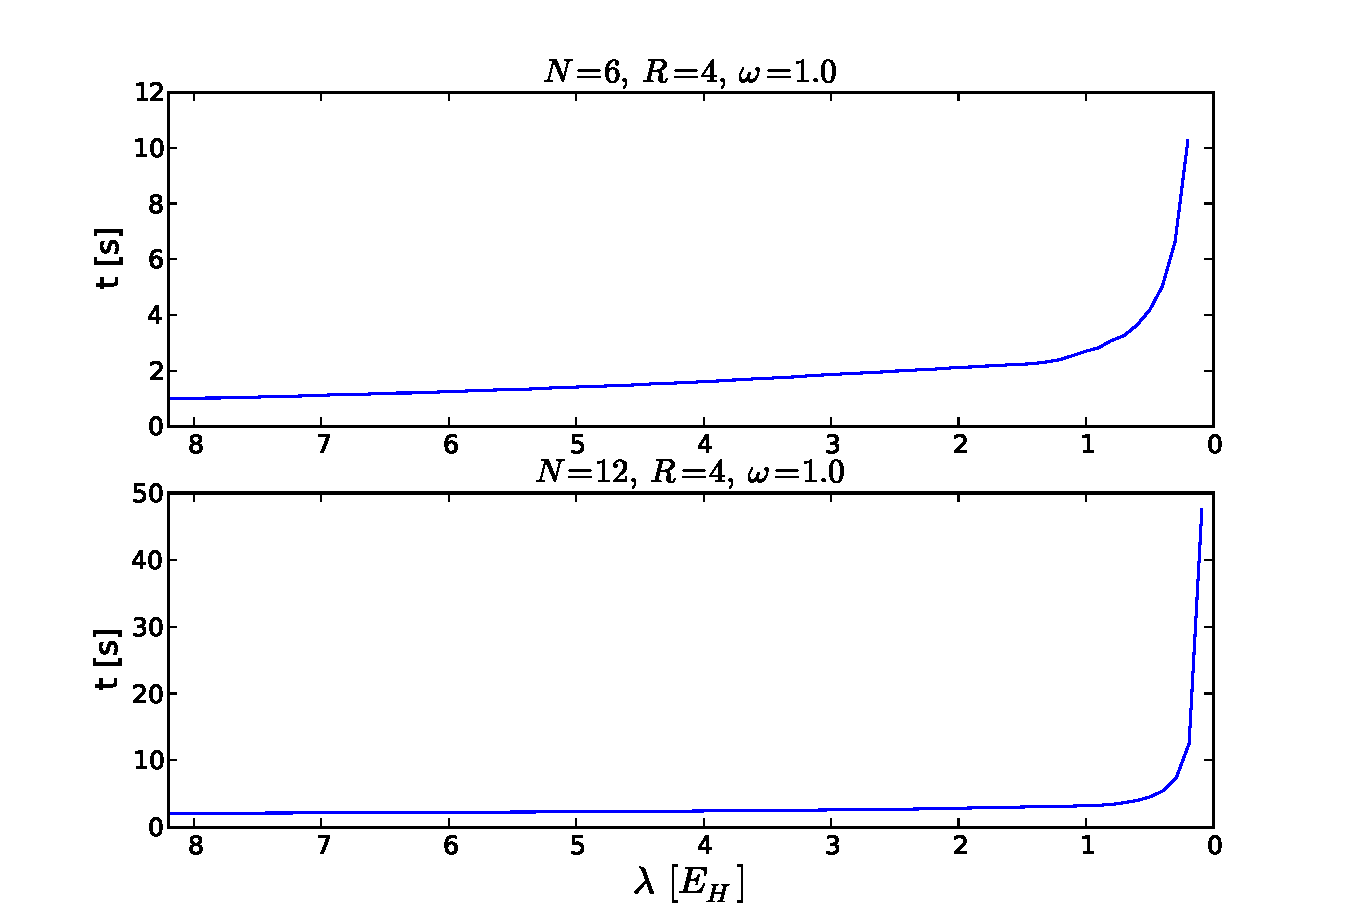
\includegraphics[scale=0.45]{../Plots/timeIMlambda.pdf}
\end{center}
\caption{Required CPU time as function of the flow parameter $\lambda$. The example is with HF basis and effective interaction. The given time includes only the integration, not setup of the system, Hartree-Fock calculation etc.}
\label{fig:timeIMlambda}
\end{figure}

Interested if the HF basis always solves the problem of numerical instabilities, we subsequently 
performed calculations with higher numbers of particles $N$.\\
For $N=12$ particles, the first results with $R\ge 5$ look quite promising, see table \ref{tab:12part0wegner}. However, during our calculations we encountered another problem, which let us restrict to very small values of $R$: Especially as the oscillator frequency $\omega$ is lowered, the system of equations gets stiff, which causes difficulties in the integration process. For well converging runs, it is usually sufficient to integrate maximally to $\lambda=0.1$ until $E_0$ has stabilized. However, for the calculations in table \ref{tab:12part0wegner} and others with $N=20,30,\dots$ particles, we need to integrate much further until convergence is reached. For the example of  $N=12, R=6,\omega=0.1$, the ground state energy $E_0$ has still not converged  for $\lambda=0.008$, see listing \ref{list:1} in the Appendix. As we already observed in figure \ref{fig:time1} for the free-space case and now again see for the in-medium approach in figure \ref{fig:timeIMlambda}, the required CPU time blows up enormously as $\lambda$ is approaching zero, even if the calculations have a comparably good convergence behaviour. The stiffness of the equations thus results in massive computational costs.\\
Moreover, for larger numbers of particles $N$, the calculations are not converging any more. When performing runs with $N=20,30,\dots$ particles in order to analyse if we encounter the same problem of stiffness, almost no calculation with $\omega\in\lbrace 0.1,0.28,0.5,1.0\rbrace$ was converging. However,  numerical stability improves as we increase the oscillator frequency $\omega$, and runs with $\omega \in \lbrace 2.0,3.0,\dots\rbrace$ are converging and generally with fewer required integration steps, see also table \ref{tab:timeConv}.


The fact that those numerical instabilities arise for larger values of $N$, as well as smaller values of $\omega$, indicates that higher correlations between the particles cause the problem and set limits to the applicability of our method.\\
Both observations, blow up of CPU time due to stiffness and non-convergence of the equations, motivated us to implement additionally White's generator and to proceed with this one for larger values of $N$.

\begin{table}
\begin{center}
\begin{tabular}{|c||c|c|c|c|c|c|c|}
\hline
$\omega$  &0.1 & 0.28& 0.5&1.0 &2.0 & 3.0 & 5.0\\
\hline
$t_{\text{Std}}$  &nc & nc&45.0 &15.1 &13.8 & 7.8 & 11.2\\
$t_{\text{Eff}}$ & nc& nc& nc& 26.9& 10.9& 6.0& 9.1\\
\hline
\end{tabular}
\end{center}
\caption{Required CPU time (in $s$)  such that the energy $E_0$ converges to six decimals. The first line lists the results with standard Coulomb interaction, the second one with effective interaction. The label ''nc'' denotes non-converging runs.}
\label{tab:timeConv}
\end{table}

\section{In-medium SRG: White's generator}
\label{sec:White}
\subsection{Motivation}
As explained in chapter \ref{chap:SRG}, White's generator introduces similar decaying speeds for all matrix elements, making numerical approaches much more efficient. Two main motivations led us to use this generator:\\
First of all, we hope to solve the problem of stiffness of the equations and to be able to get converging results for systems with higher correlations, too. Second, 
 as we have shown in section \ref{sec:ImplIMSRG},
White's generator is computationally much more efficient. Since the generator focuses on zeroing out the one-particle-one-hole and two-particle-two-hole excitations connected to the ground state $\left| \Phi_0 \right\rangle$, the only non-vanishing terms are one-body terms of the form $\eta_{ph}^{(1)}$ and two-body terms of the form $\eta_{pphh}^{(2)}$, where $p$ denotes particles and $h$ holes.
Making use of these properties, an effective implementation can simplify Eqs. (\ref{eq:flow2order1})-(\ref{eq:flow2order}) quite a lot, considerably reducing the number of required floating point operations. Apart from better stability, we therefore expect our calculations to take less CPU time, which is of special importance as we want to increase the number of particles $N$ and single-particle states in our basis.

We proceed the following way: After validating our code, we will compare the convergence behaviour of the SRG method with both, Wegner's and White's, generator . Particularly, we will look at how the required CPU time is changed, indicating the number of integration steps and therefore being a measure for the stiffness of the equations. Afterwards, we will analyse how numerical stability is affected.\\
If the results are satisfying, we continue our calculations with larger ranges of particles $N$ and shells $R$ and study how well applicable our method is for those systems, comparing with other many-body methods.


\subsection{Code validation}
In accordance with the other implementations, we first performed a number of test calculations in order to be sure that the code is free of bugs. In this case, it makes sense to take the same tests as we did for Wegner's generator: Including additionally the loop term terms of higher order interactions, IM-SRG(2) should be exact for $N=2$ particles and yield the same ground state energy $E_0$ as the free-space approach and exact diagonalization.\\
The results are listed in table \ref{tab:CompIMWhite}, where we performed calculations with HO as well as HF basis. We observe that exactly the same results are obtained, indicating that the code is working correctly.

\begin{table}
\begin{center}
\begin{tabular}{ccccc}
\hline\hline
 & & \multicolumn{2}{c}{IM-SRG(2/3) White} & \\
$\omega$ & $R$ & HO basis & HF basis & Free space SRG \\
\hline
0.1 & 3 &0.442188760 &0.442188760&0.442188760  \\
& 5 & 0.441613707 &0.441613707& 0.441613707\\
& 7 &0.441329736 & 0.441329736 & 0.441329736\\
\hline
0.28 & 3&1.03268141 &1.03268141 &1.03268141 \\
& 5&1.02658806 &1.02658806 & 1.02658806\\
& 7&1.02470588 & 1.02470588 & 1.02470588 \\
\hline
0.5&3 &1.68163200 &1.68163200 &1.68163200 \\
& 5&1.66949822 &1.66949822 &1.66949822 \\
& 7&1.66579935 &1.66579935 &1.66579935 \\
\hline
1.0 & 3&3.03860458 &3.03860458 &3.03860458 \\
& 5 &3.01760623 &3.01760623& 3.01760623\\
& 7 &3.01101998 &3.01101998& 3.01101998\\
\hline\hline
\end{tabular}
\caption{Comparison of the ground state energy $E_0$ in free space and IM-SRG(2/3) for $N=2$ particles. With IM-SRG(2/3) we denote second-order IM-SRG(2), extended by the loop terms of three-body interactions. The high number of specified digits shall emphasize that exactly the same result is obtained. All runs have been performed with standard Coulomb interaction.}
\label{tab:CompIMWhite}
\end{center}
\end{table}

\subsection{Comparison with Wegner's generator}
\label{subsec:CompWegner}
As mentioned above, we expect the calculations with White's generator to require less CPU time than the ones with Wegner's generator. The first reason is that the flow equations simplify due to the properties of $\hat{\eta}$, the second reason is that we assume the equations not to be stiff any more, reducing the number if integrations steps. With the number of integration steps as well as the number of floating-point operations per step reduced, we hope for a considerable reduction of CPU time. \\
Figure \ref{fig:timeWhiteWegner} shows that our assumptions are right: The calculations with White's generator do indeed require much less time . This seems to be more pronounced as the number of \mbox{shells $R$} is increasing, which can be explained by the fact that the simplification of the flow equations has greater impact as the number of single-particle states is increasing.\\
Another important observation is that the huge blow up of time for small values of $\lambda$, which we faced with Wegner's generator, no longer exists to the same extent.
This indicates that the equation system is not stiff any more and exhibits better numerical properties, making it more straightforward to solve with the ODE solver.
 
\begin{figure}
\begin{center}
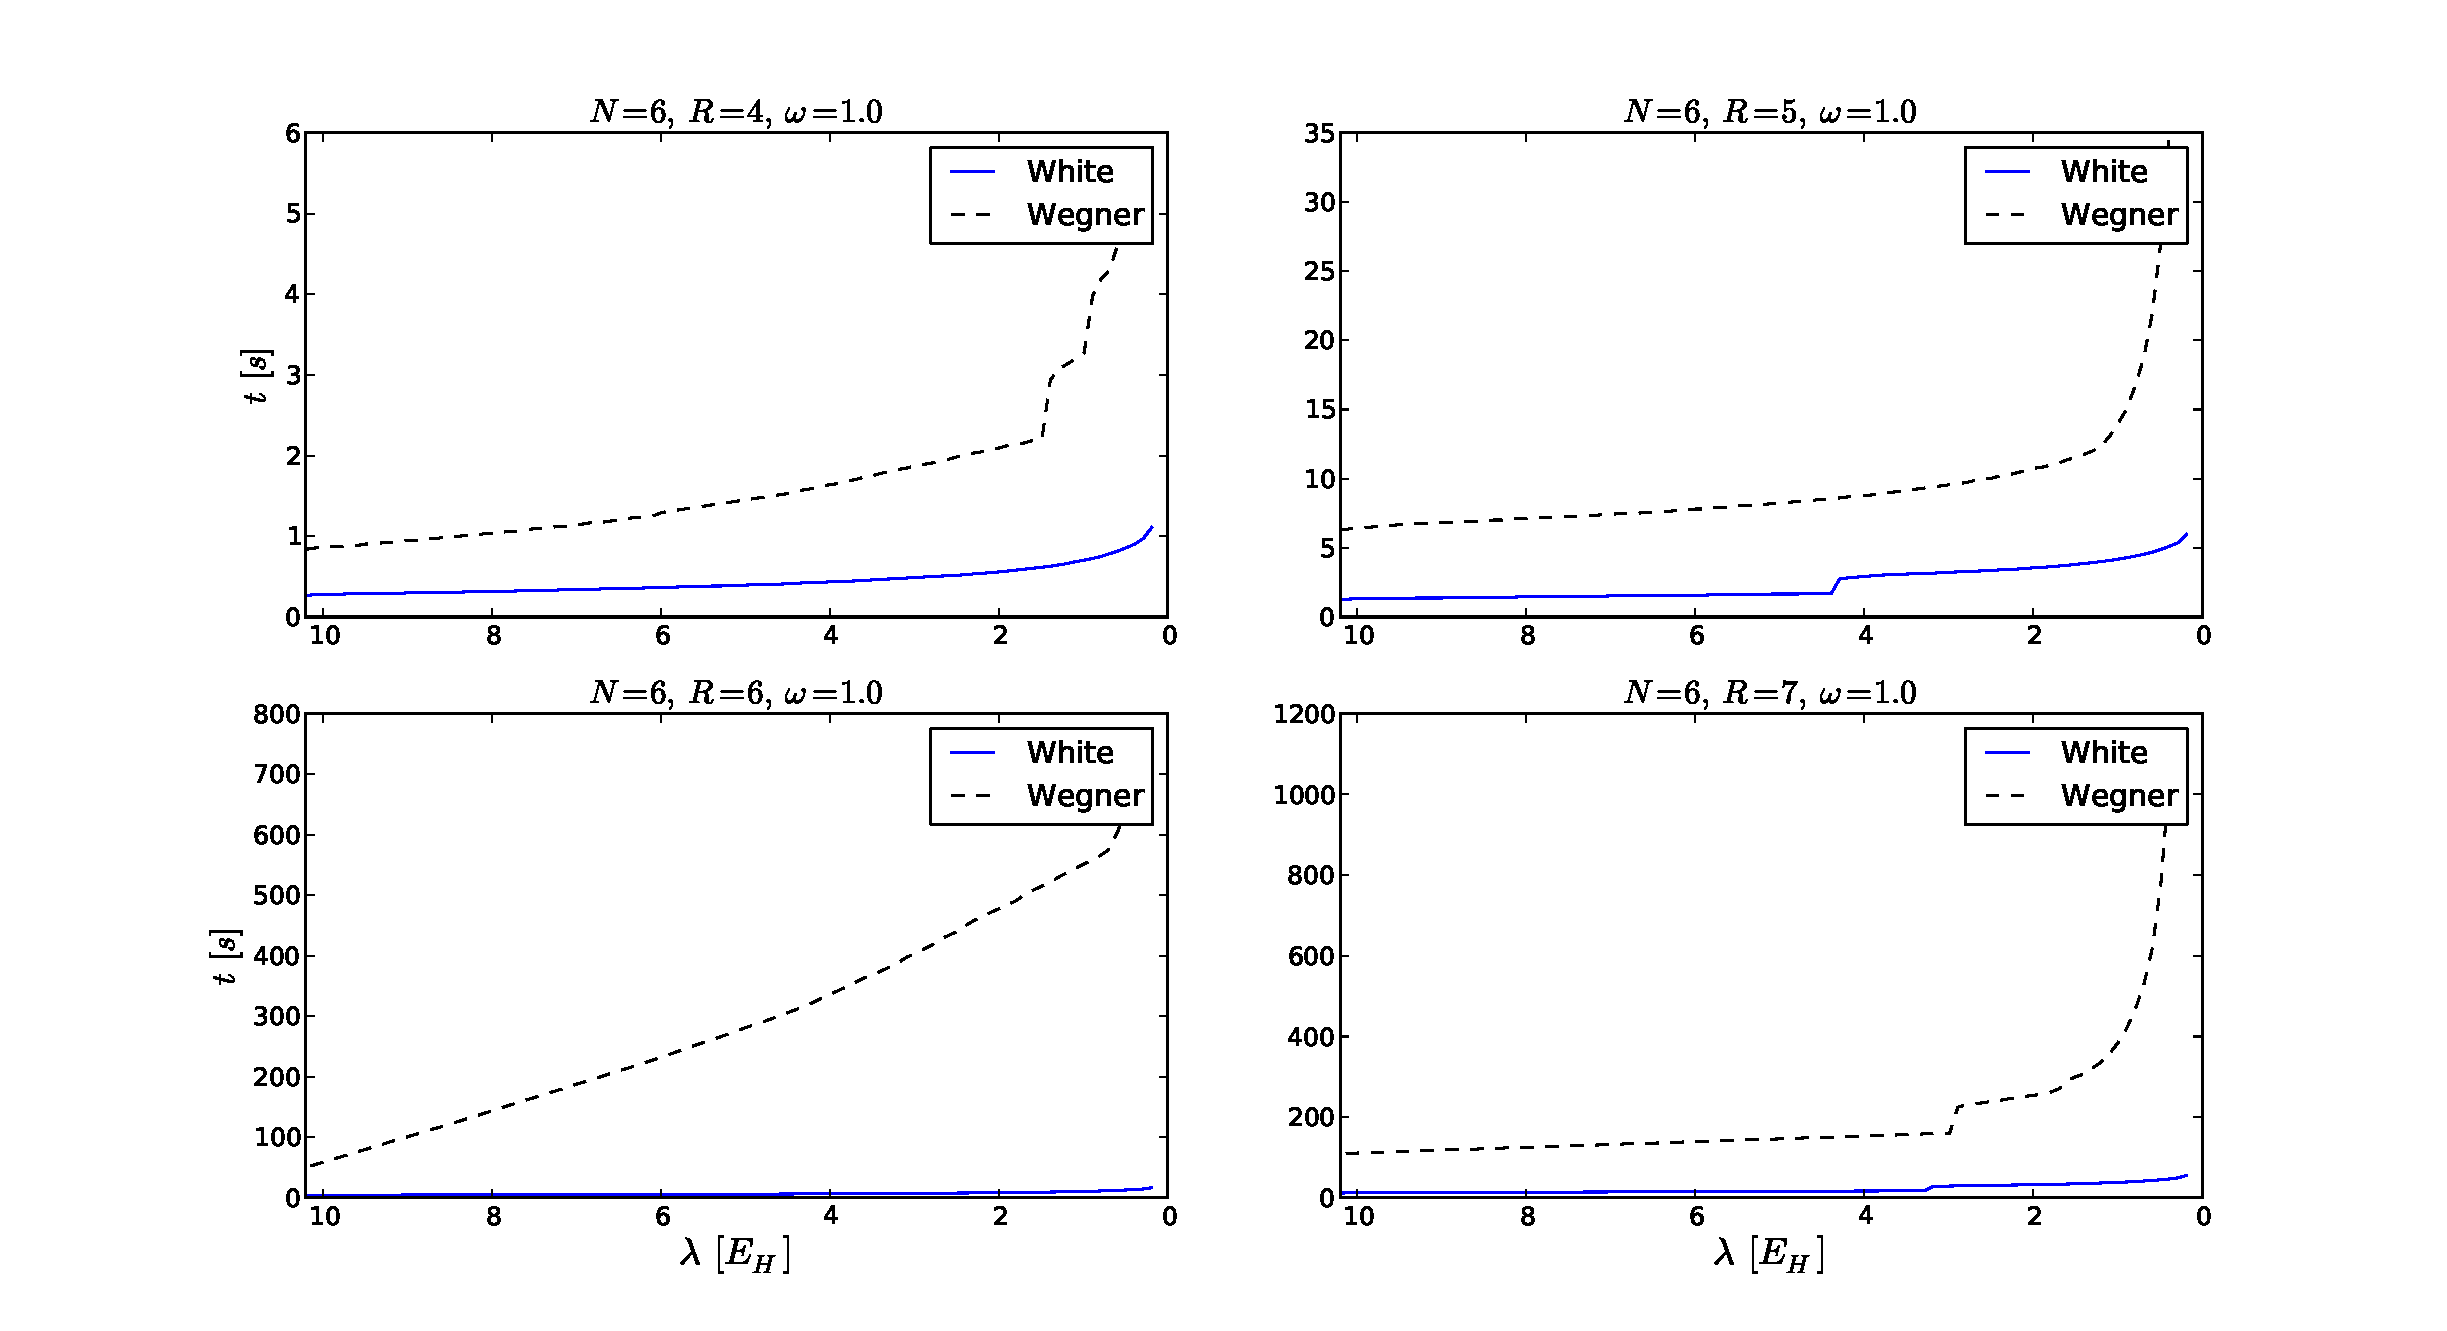
\includegraphics[scale=0.42]{../Plots/timeWhiteWegner.pdf}
\caption{Required CPU time on $p=1$ processor for SRG calculations performed with White's and Wegner's generator. The runs have been performed with HF basis and standard interaction. To give a reasonable comparison, the time does only consider the integration of the flow equations, not setup of the system, Hartree-Fock calculation etc.}
\label{fig:timeWhiteWegner}
\end{center}
\end{figure}

\begin{figure}
\begin{center}
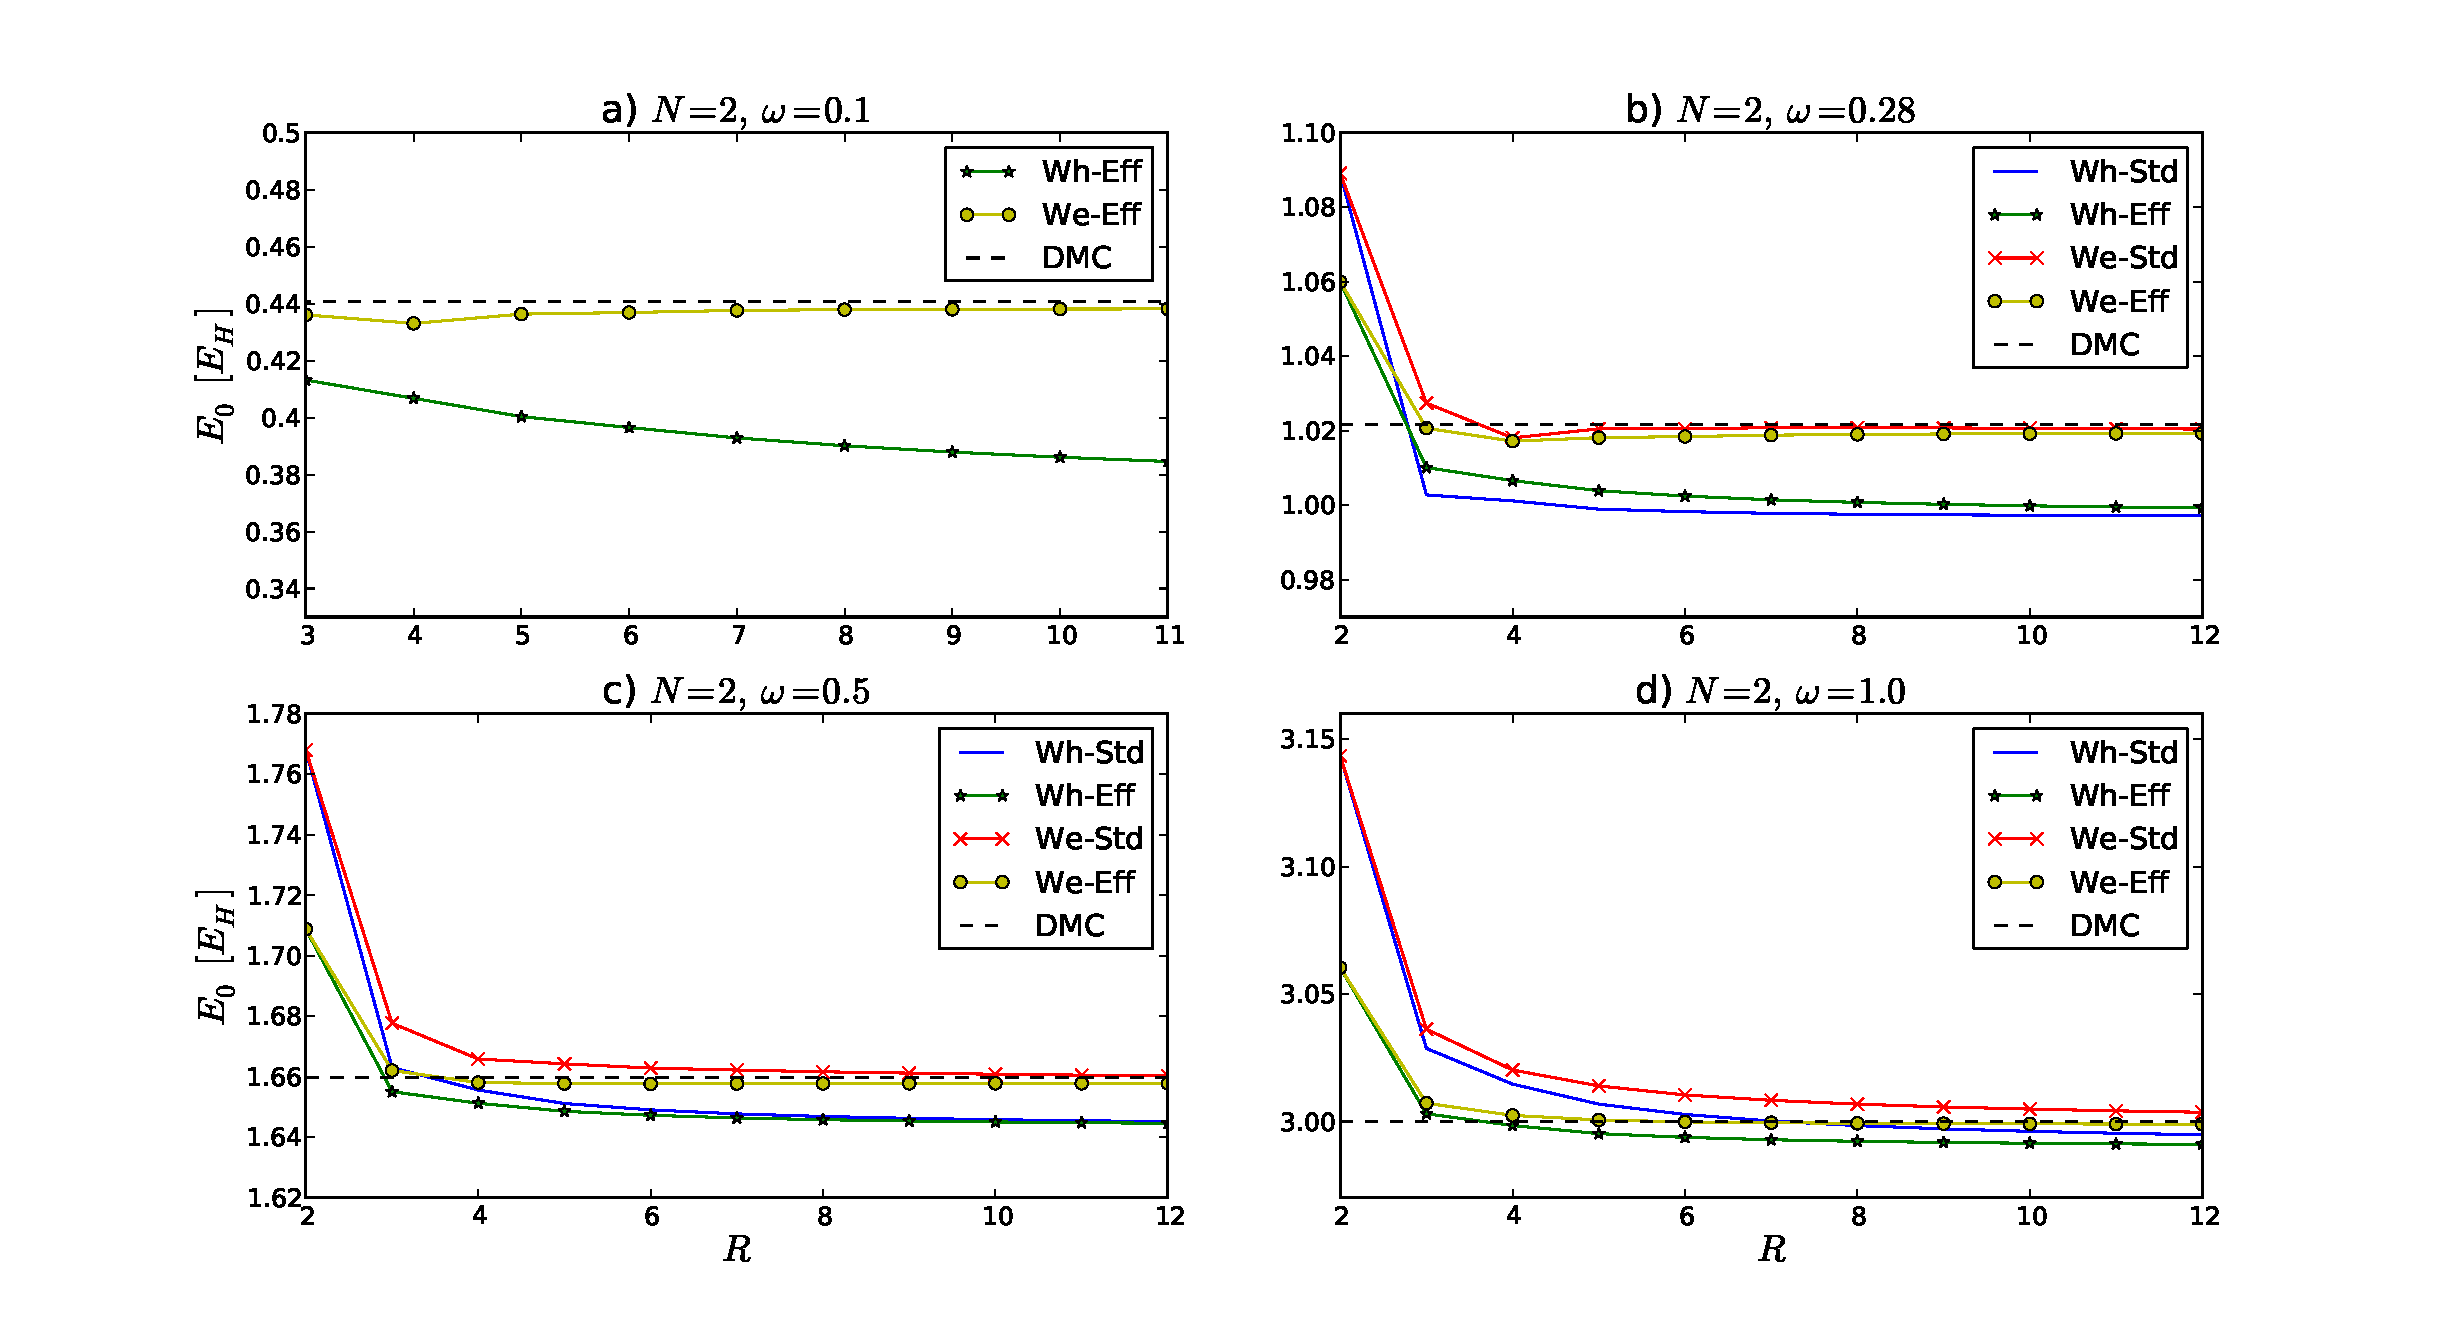
\includegraphics[scale=0.42]{../Plots/compWhiteWegner2.pdf}
\end{center}
\caption{Comparison of the convergence behaviour as function of the shell number $R$ with Wegner's generator, standard interaction (We-Std) and effective interaction (We-Eff), and White's generator with standard (Wh-Std) and effective interaction (Wh-Eff). All runs have been performed with $N=2$ particles and Hartree-Fock basis. For benchmarking, we have also plotted the ground state energy we got with Diffusion Monte Carlo (DMC). }
\label{fig:compWhiteWegner2}
\end{figure}

\begin{figure}
\begin{center}
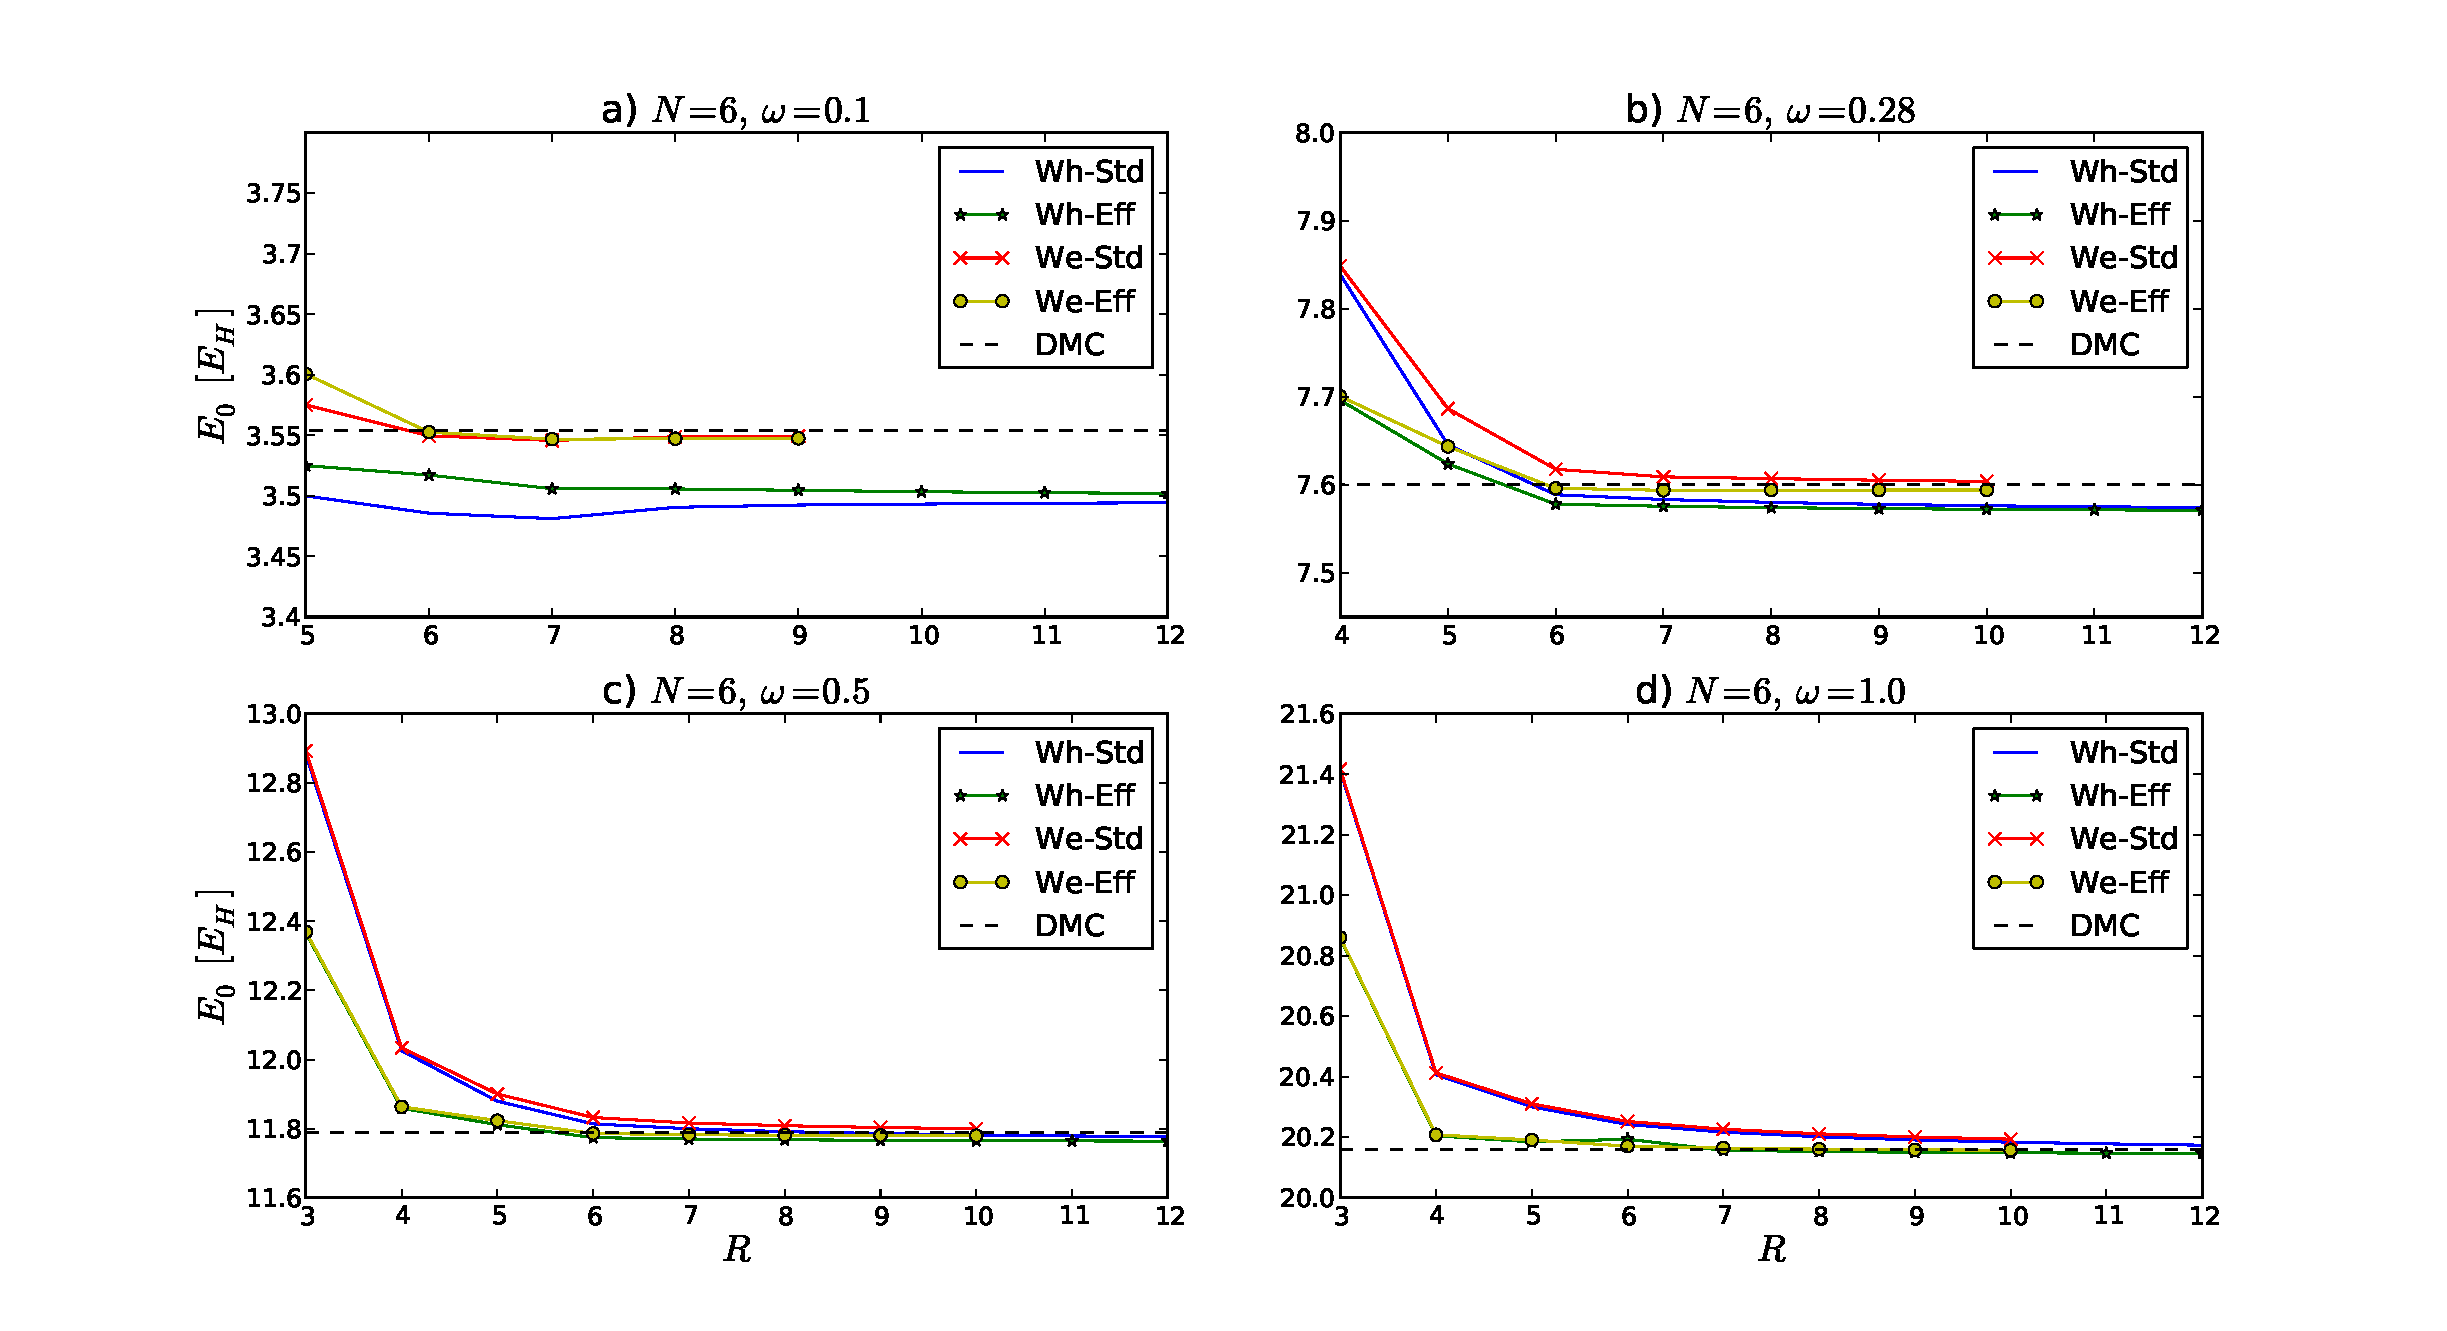
\includegraphics[scale=0.42]{../Plots/compWhiteWegner6.pdf}
\end{center}
\caption{Comparison of the convergence behaviour as function of the shell number $R$ with Wegner's generator, standard interaction (We-Std) and effective interaction (We-Eff), and White's generator with standard (Wh-Std) and effective interaction (Wh-Eff). All runs have been performed with $N=6$ particles and Hartree-Fock basis. For benchmarking, we have also plotted the ground state energy we got with Diffusion Monte Carlo (DMC). }
\label{fig:compWhiteWegner6}
\end{figure}

Another interesting aspect is how the numerical results compare with each other. For $N=2$ particles, figure \ref{fig:compWhiteWegner2} illustrates that Wegner's generator generally gives a better approximation to the ground state energy $E_0$. A similar trend can be observed for $N=6$ particles and low values for $\omega$ in figure \ref{fig:compWhiteWegner6}. In these cases, the results with White's generator are constantly slightly too low, suggesting that due to truncation, systematically a positive term is omitted. However, as the number of particles $N$ and oscillator frequency $\omega$ is increased, the approximation seems to get better.

Since the flow equations with Wegner's generator get stiff and often do not converge as the number of particles $N$ is increased, we continue our larger computations with this generator. The full results of the IM-SRG(2) calculations with White's generator can be found in Appendix \ref{App:AppendixA}. Since calculations with a HF basis generally result in a smaller error, all the runs have been performed with a preceding Hartree-Fock calculation.

\begin{table}
\begin{center}
\begin{tabular}{l|l|l|l|l|l}
\hline
$R$& 5 &7 & 10 & 12& 15\\
\hline
$n$ & 6640\, &57602\, &613572\, &2092438\, & 9495322\, \\
\hline
\end{tabular}

\begin{tabular}{l|l|l|l|l}
\hline
$R$& 17&  20 &22&  25 \\
\hline
$n$ & 22274038 & 67647814& 130003774 & 312789734 \\
\hline
\end{tabular}
\end{center}
\caption{Number of coupled ordinary differential equations $n$ that have to be solved for $N=2$ particles.}
\label{tab:numlig}
\end{table}

To get an impression of the dimension of the problem to be solved, table \ref{tab:numlig} lists the number of ordinary differential equations to be solved for the example of $N=2$ particles. It gets evident that for each additional included shell $R$, the number of equations is considerably increased, which of course is reflected in the required CPU time. For this reason, we restricted us to maximally $N=20$ shells, although we in principle could have treated larger basis sizes, too. However, as we would neither get any new insights into the physics of the systems, nor in the SRG method itself, we think that $R=20$ shells is a reasonable limit. It provides all information needed to analyse the convergence behaviour as function of $R$, which we will come back to in the next section.\\
It should be mentioned that the number of differential equations is nearly independent of the number of particles $N$, and that more or less just the number of included shells $R$ determines the size of the problem. However, for a larger number of particles, our model space is larger, too, suggesting that we need to integrate over a longer interval. Therefore the number of integration steps is increased, which requires additional CPU time, see table \ref{tab:cputime}.

\begin{table}
\begin{center}
\begin{tabular}{ccccc}
\hline\hline
$N$ & $R=10$ & $R=14$ & $R=16$ & $R=20$ \\
\hline
2 & 0.36 &0.9 &2.3 & 10.2 \\
6 &0.9 &5.1 & 11.9& 74.6 \\
12 &2.8 &22.7 &50.6 &182.7 \\
20 &11.8 & 30.9&108.4 & 659.8\\
\hline\hline
\end{tabular}
\end{center}
\caption{Required CPU time (in hours) for runs with $\omega=1.0$, Hartree-Fock basis and effective interaction. Here, we used the computing cluster ''Abel'', the Linux cluster at the University of Oslo-}
\label{tab:cputime}
\end{table}

\subsection{Comparison with other many-body methods}
In the following, we will examine how our SRG results behave as function of shells $R$ and rate them with respect to other many-body methods. In doing so, we will consider the following methods: 
\begin{itemize}
\item \textbf{Hartree-Fock} (HF): The HF code is written by us and precedes the SRG calculation, such that we can use a HF basis. Regarding theoretical aspects of the method, we refer to section \ref{sec:HF}.
\item \textbf{Diffusion Monte Carlo} (DMC): We developed an own DMC code, independently of the SRG implementation. As explained in section \ref{sec:DMC0}, this quantum Monte Carlo method solves Schr\"odinger equation using a Green's function.
\item \textbf{Full Configuration Interaction} (FCI): These results are supplied by the former master's student F. B. Olsen, see \cite{Frank}. For a given number of single-particle \mbox{states $n_{sp}$}, FCI includes all  possible Slater determinants, which are obtained by exciting
 particles from the ground state configuration to all possible virtual orbitals.  Within this basis, the eigenvalues of the full Hamiltonian are computed. \\
 Since for a given Hamiltonian, the method is exact within the space spanned by the basis functions, FCI is a valuable benchmark for our results. However, only systems with rather small numbers of included shells $R$ can be compared, since the number of determinants in the basis grows factorially with the number of particles and orbitals. For $N$ electrons in $n_{sp}$ single-particle states, the Hilbert space has dimension
 \[
 \text{dim}(\mathcal{H}) = \binom{n_{sp}}{N}.
 \]
For an example of $N=12$ electrons and $R=10$ shells, which is still one of the smaller systems considered by us, one would have about $3.5\cdot 10^{15}$ possible Slater determinants, which is beyond the limit of current FCI calculations \cite{Shimizu:2012rt}. The largest system run here, with $N=30$ particles and $R=20$ shells, corresponding to $420$ basis functions, yields approximately $6.5\cdot 10^{45}$ determinants, which is much too large for an exact diagonalization.
\item \textbf{Coupled Cluster}: The coupled cluster data we compare our results with, are supplied by the former master's student C. Hirth, see \cite{Christoffer}. The method aims to solve the time-independent Schr\"odinger equation using an exponential ansatz for the wave function,
\be 
|\Psi\rangle \equiv e^{\hat{T}}|\Phi_0\rangle,
\label{eq:CCWF}
\ee
where $|\Phi_0\rangle$ is a reference Slater determinant and $\hat{T}$  the cluster operator  including all possible excitations. If the excitations are sorted by the number of excited electrons, $\hat{T}$ can be expressed as sum of a one-particle one-hole (single excitations) operator, two-particle two-hole (double excitations) operator etc.
\[
\hat{T} = \hat{T}_1 + \hat{T}_2 + \hat{T}_3 + \dots
\]
A common approach, called CCSD and used by C. Hirth, is to only include singles and doubles, such that Eq.~(\ref{eq:CCWF}) simplifies to
\[
|\Psi\rangle \approx e^{\hat{T}_1 + \hat{T}_2} |\Phi_0\rangle.
\]
This ansatz for the wave function is now used to iteratively solve Schr\"odinger's equation. For more details concerning the setup and solution of the coupled cluster equations, we refer to\cite{shavitt2009many}. \\
The advantage of CCSD over FCI is that much larger systems can be treated, which gives us a reference method where no FCI data are available. Moreover, CCSD is subject to truncation, similar to IM-SRG(2), giving a good starting point to compare the errors made by the different methods.

\end{itemize}

Figures \ref{fig:compall0} to \ref{fig:compall2} show our IM-SRG(2) results as functions of the shell number $R$ and compare them with other many-body methods. First, we consider oscillator frequency $\omega=1.0$, afterwards we look at lower values for $\omega$.\\
A first important observation is that with increasing $R$, the ground state energy $E_0$ is decreasing and seems to converge.
For the comparison with other methods, let us start with the Hartree-Fock calculations:\\
Evidently, SRG performs much better. The curve of the Hartree-Fock results lies considerably more off the ones of FCI and DMC than our SRG curve does. This meets our expectations, since Hartree-Fock calculations only consider one-particle one-hole excitations, while we also take two-particle two-hole excitations into account. \\
A next interesting point is how SRG compares to FCI, which can be regarded as exact for a given value of $R$: Our results lie systematically slightly below the FCI results, suggesting that a postive term is omitted when truncating to IM-SRG(2). Since FCI is limited to rather small basis sizes, we have unfortunately not that many data for comparison available. \\
However, for larger values of $R$, we can evaluate our results with respect to DMC and CCSD calculations. In general, the deviation of the SRG from the DMC results are comparable with the ones of CCSD. For larger number of particles, SRG seems even to perform slightly better. However, it is important to remark that also DMC only serves as  guideline and does not give the exact result, since it is subject to errors like the fixed-node approximation. For a direct comparison between SRG and CCSD, up to $N=30$ particles, we also refer to table \ref{tab:compCCSD} in Appendix \ref{App:AppendixA}. \\
For lower values of the oscillator frequency $\omega$, that is higher correlations, the deviations of the SRG to the DMC and FCI results get larger, but they still stay comparable to CCSD. In general, the calculations with standard interaction perform slightly better than the ones with effective interaction. One should note that CCSD, although truncated to single and double excitations, implicitly includes higher excitations, too. This arises from the exponential ansatz and explains the overall good performance of the method. \\
Essentially, our SRG results compare really well with  the other many-body methods. In particular when comparing to Hartree-Fock, it gets evident how important the contributions of two-particle two-hole excitations are. Obviously, they are much larger than the corrections coming from higher excitations, which supports our choice to truncate the SRG equations on a two-body level. Expanding our method to IM-SRG(3), IM-SRG(4), etc. is in principle straightforward, and we would then expect to lie even closer to the FCI evaluations. As shown before, for $N=2$ particles, already including the loop terms of three-body interactions is enough to obtain those exact results. \\
A full listing of all our results, up to $N=42$ particles, can be found in Appendix \ref{App:AppendixB}.

\begin{table}
\begin{center}
\begin{tabular}{|c|c|c c c|c c c|}
\hline
\multicolumn{2}{|c|}{} &\multicolumn{3}{|c|}{$\omega=1.0$} &
 \multicolumn{3}{|c|}{$\omega=0.28$}\\
$N$ & $R$ & SRG & FCI& $\Delta_{FCI}$ & SRG & FCI& $\Delta_{FCI}$ \\
\hline
2 & 5 & 3.0068 & 3.0176 & 0.0108 (0.36\%) &0.9990 & 1.0266 &  0.0276 (2.69\%) \\
  & 8 & 2.9984 & 3.0092 & 0.0108 (0.36\%) &0.9976 & 1.0242 &  0.0266 (2.60\%)\\
 & 10 & 2.9961 & 3.0069 & 0.0108 (0.36\%) &0.9973 & 1.0218 & 0.0245 (2.40\%) \\
 & 20 & 2.9923 & 3.0030 & 0.0107 (0.36\%) &0.9971 & 1.0225 &  0.0254 (2.48\%) \\
\hline
6 & 5 &20.3009 & 20.3167 & 0.016 (0.078\%)&7.6456 & 7.7105 & 0.0648 (0.84\%)\\
  & 8 &20.2020 & 20.2164 & 0.014 (0.071\%) &7.5802 & 7.6155 & 0.0353 (0.53\%)\\
\hline\hline
\end{tabular}
\end{center}
\caption{Comparison between the ground state energy $E_0$ (in $[E_H]$) obtained with SRG and FCI \cite{Frank}, both with standard interaction. In the column labelled with $\Delta_{FCI}$ we give the absolute and relative difference, $\left|E_{0(SRG)}-E_{0(FCI)}\right|$ and $\left|E_{0(SRG)}-E_{0(FCI)}\right|/E_{0(FCI)}$, respectively.}
\end{table}

\begin{figure}
\begin{center}
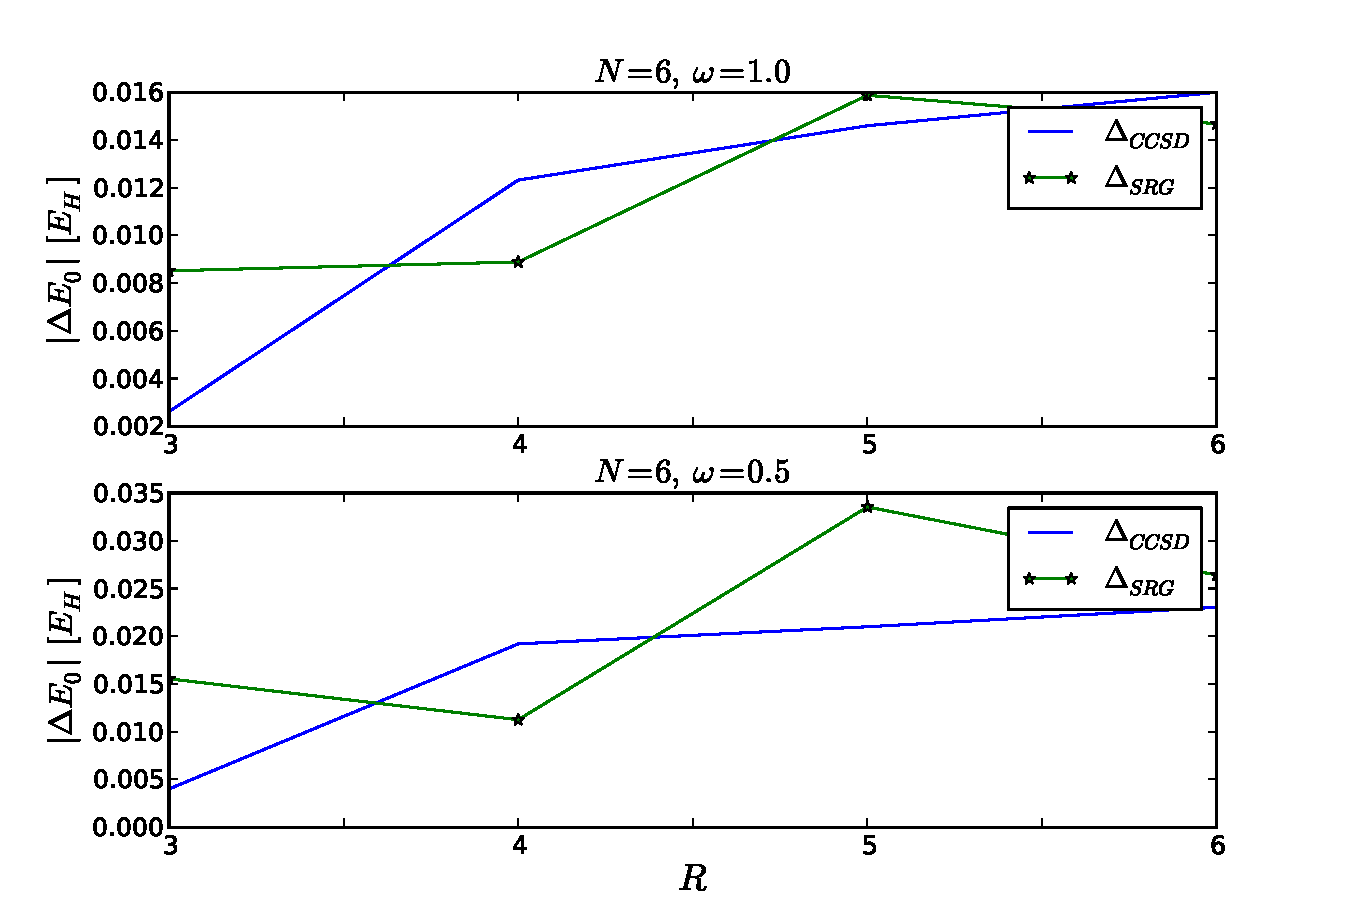
\includegraphics[scale=0.4]{../Plots/compCCSDSRG.pdf}
\caption{Difference of the ground state energy $E_0$ from the obtained DMC result. For the Coupled Cluster result, this difference is given by $\Delta_{CCSD} = |E_{0(CCSD)}-E_{0(DMC)}|$, with an analogous expression for the SRG result. The runs have been performed with standard interaction and Hartree-Fock basis. The CCSD results are taken from \cite{Christoffer}.}
\end{center}
\end{figure}


\begin{figure}
\begin{center}
\mbox{\subfigure[$N=2, \omega=1.0$, Std. interaction]{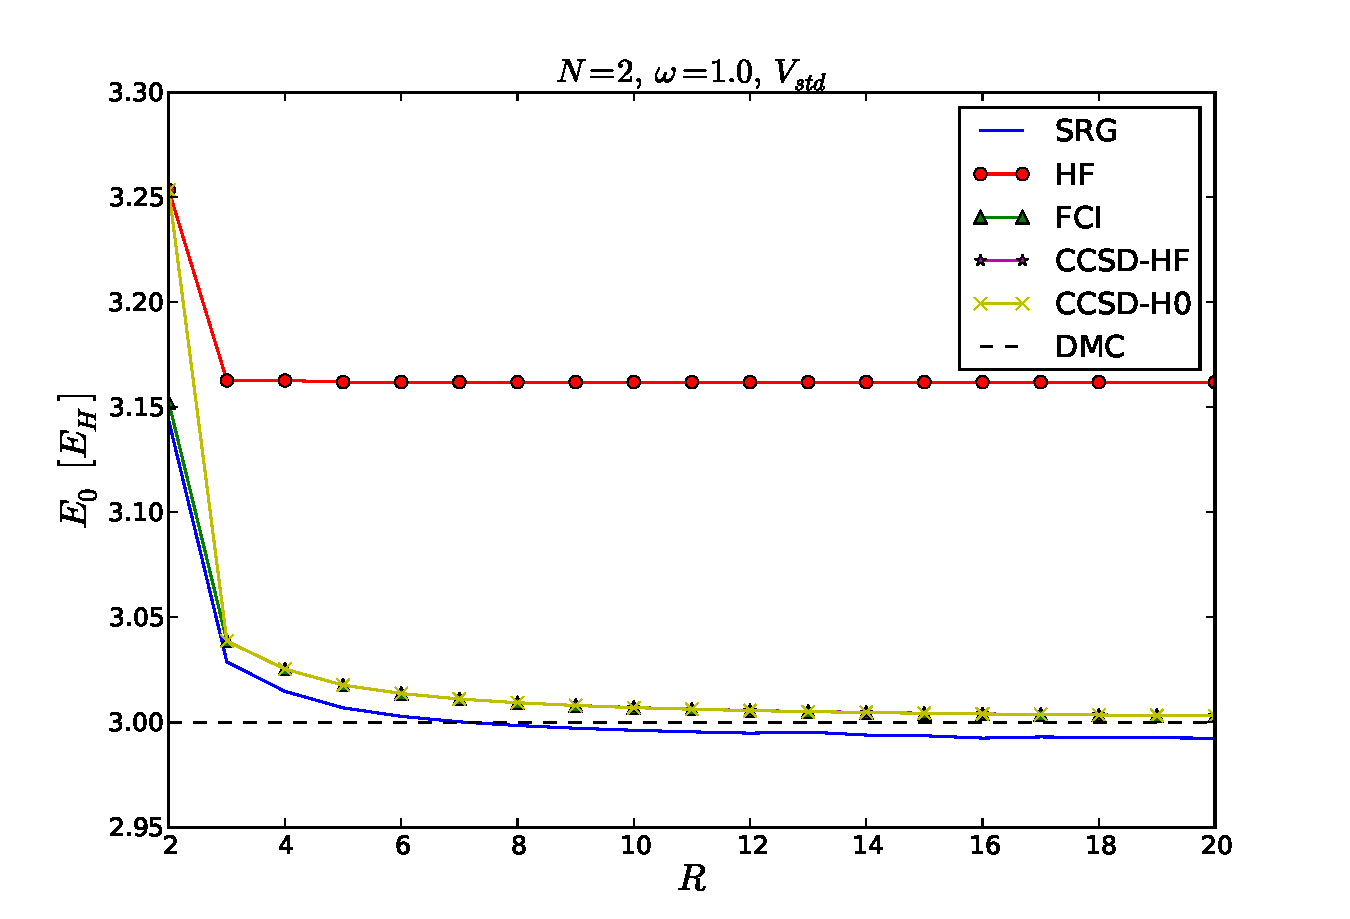
\includegraphics[scale=0.34]{../Plots/comp2partstd.pdf}}
\subfigure[$N=2, \omega=1.0$, Eff. interaction]{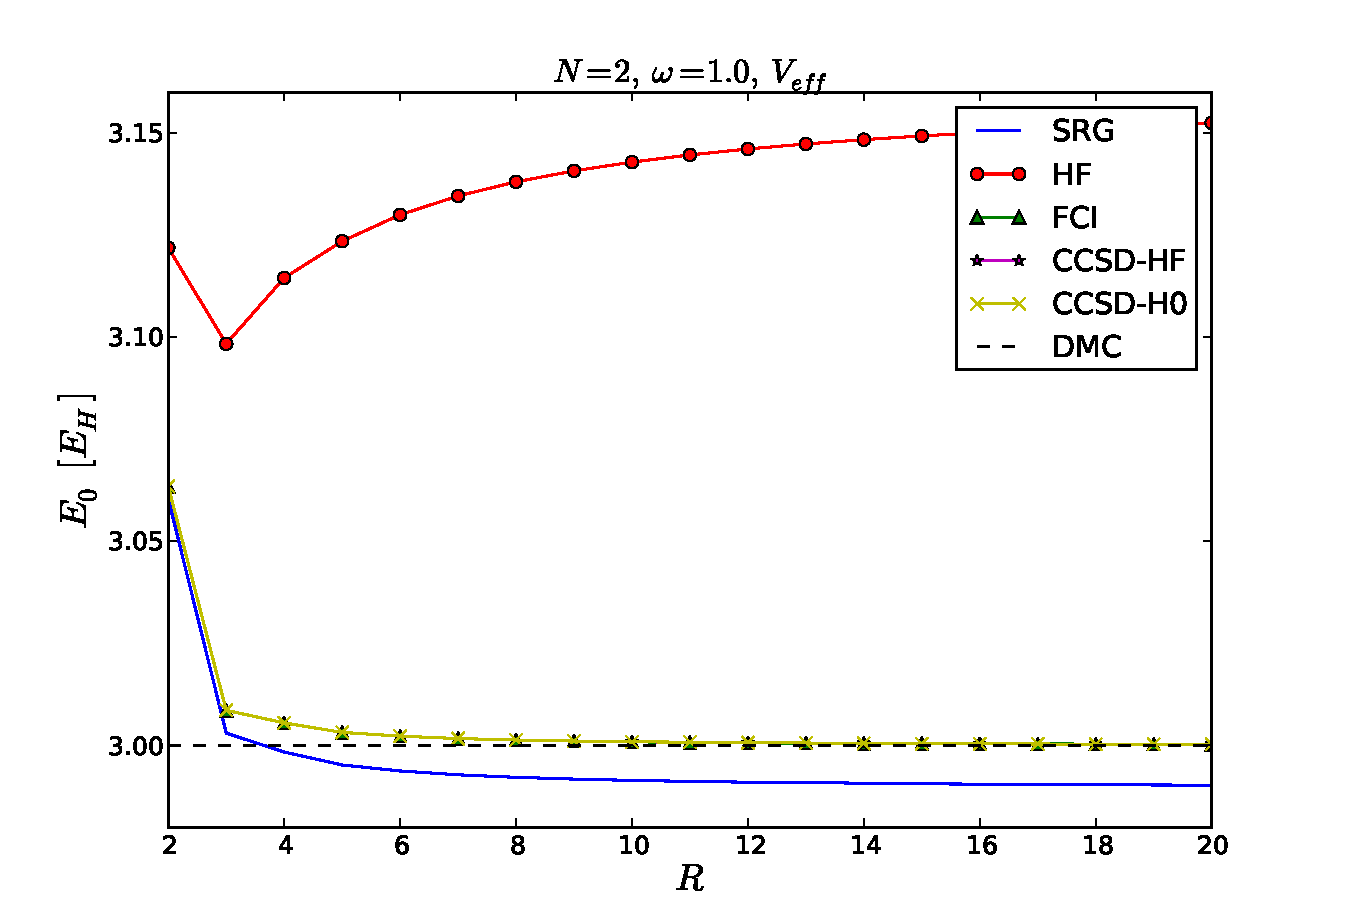
\includegraphics[scale=0.34]{../Plots/comp2parteff.pdf}}}
\mbox{\subfigure[$N=6, \omega=1.0$, Std. interaction]{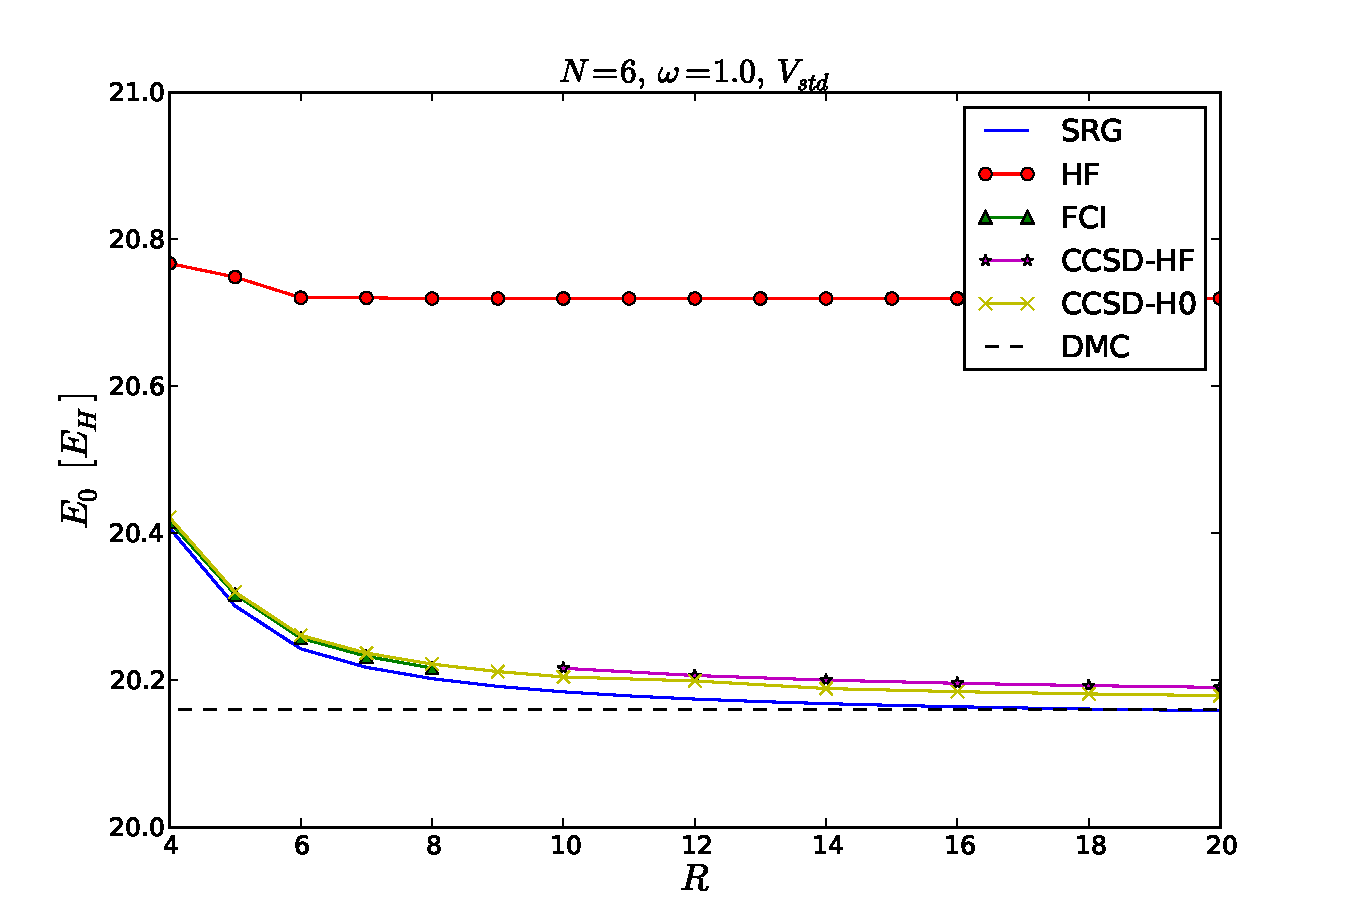
\includegraphics[scale=0.34]{../Plots/comp6partstd.pdf}}
\subfigure[$N=6, \omega=1.0$, Eff. interaction]{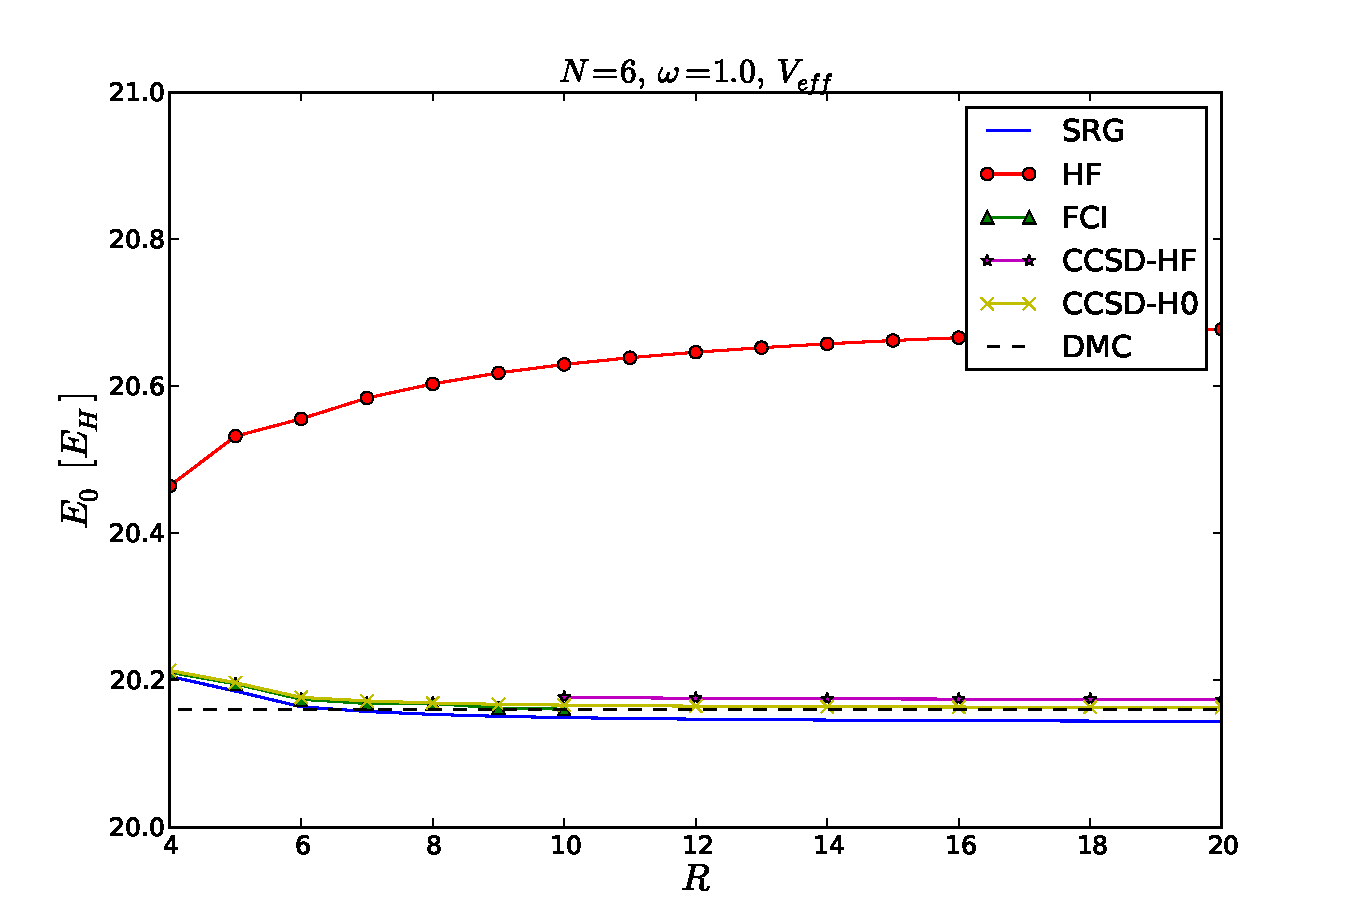
\includegraphics[scale=0.34]{../Plots/comp6parteff.pdf}}}
\mbox{\subfigure[$N=12, \omega=1.0$, Std. interaction]{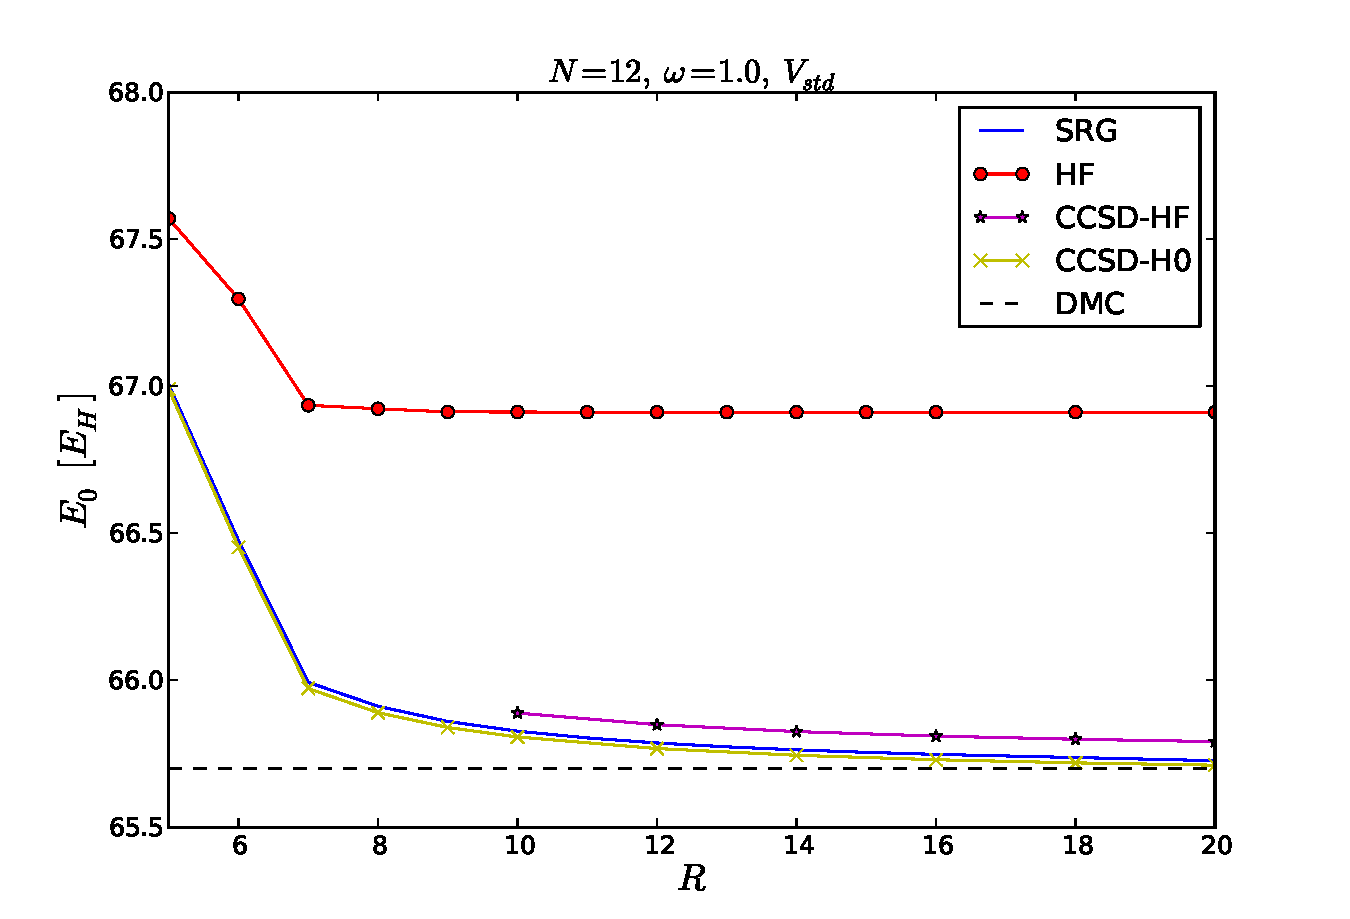
\includegraphics[scale=0.34]{../Plots/comp12partstd.pdf}}
\subfigure[$N=12, \omega=1.0$, Eff. interaction]{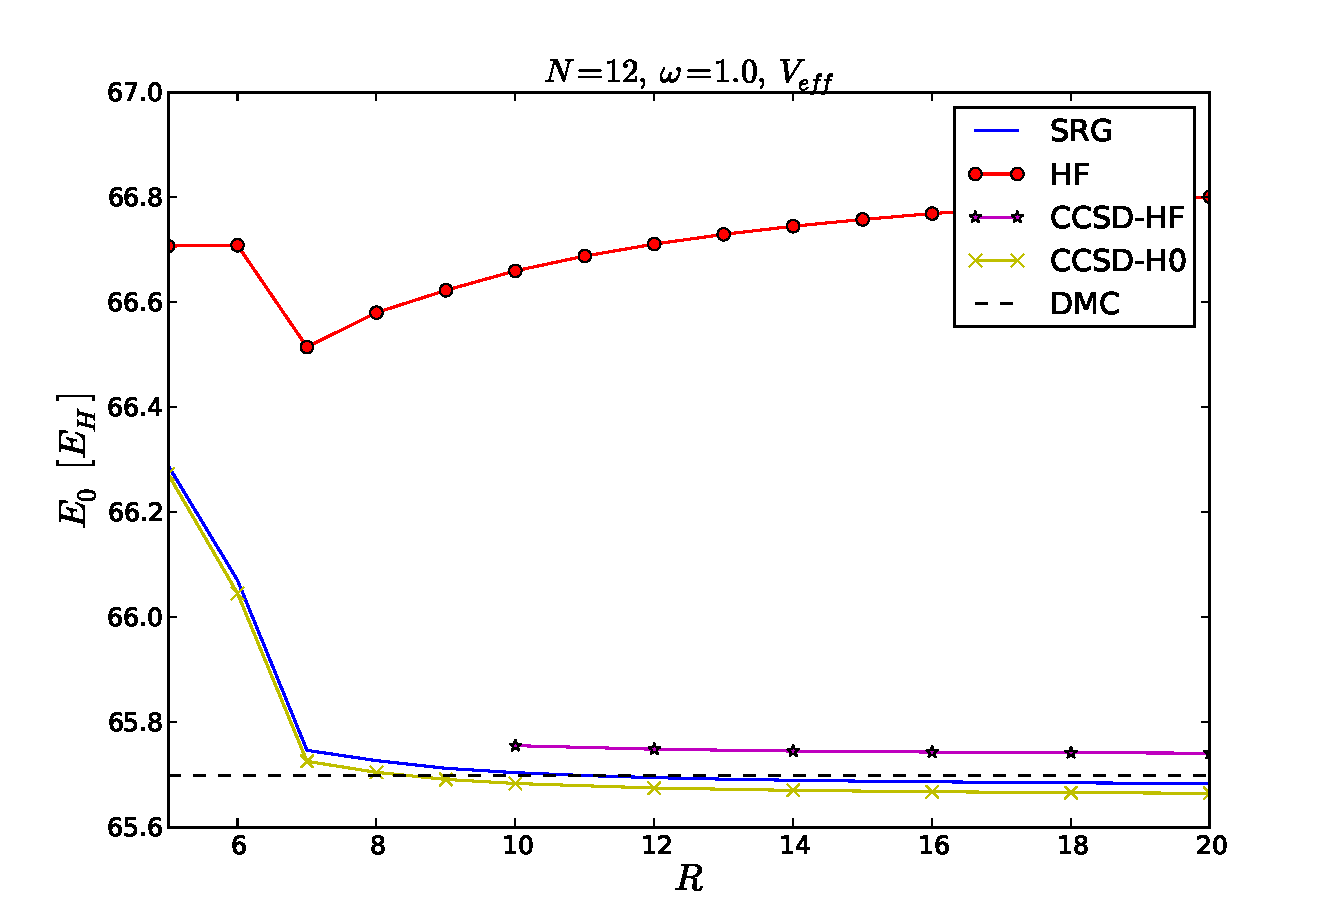
\includegraphics[scale=0.34]{../Plots/comp12parteff.pdf}}}
\end{center}
\caption{Comparison of our SRG results with other many-body methods. We performed the SRG calculations (IM-SRG(2)) with White's generator and a Hartree-Fock basis. The Hartree-Fock (HF) and Diffusion Monte Carlo (DMC) results have been obtained with code developed with us. The Full Configuration Interaction (FCI) results are taken from \cite{Frank} and the Coupled Cluster (CCSD) results from \cite{Christoffer}. The Coupled Cluster calculations include singles and doubles and are plotted both with harmonic oscillator basis (CCSD-HO) and Hartree-Fock basis (CCSD-HF). }
\label{fig:compall0}
\end{figure}

\begin{figure}
\begin{center}
\mbox{\subfigure[$N=20, \omega=1.0$, Std. interaction]{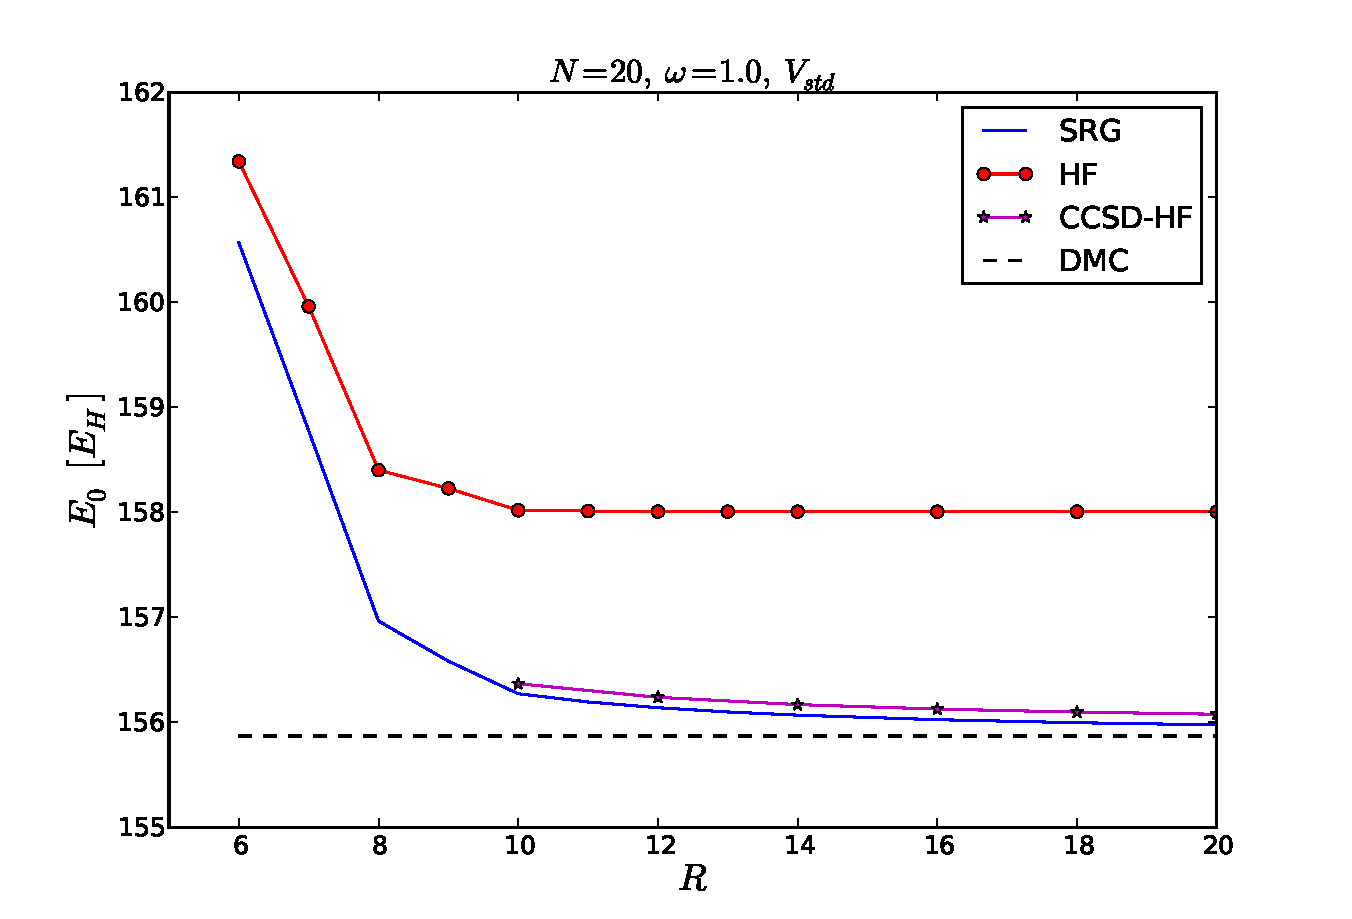
\includegraphics[scale=0.34]{../Plots/comp20partstd.pdf}}
\subfigure[$N=20, \omega=1.0$, Eff. interaction]{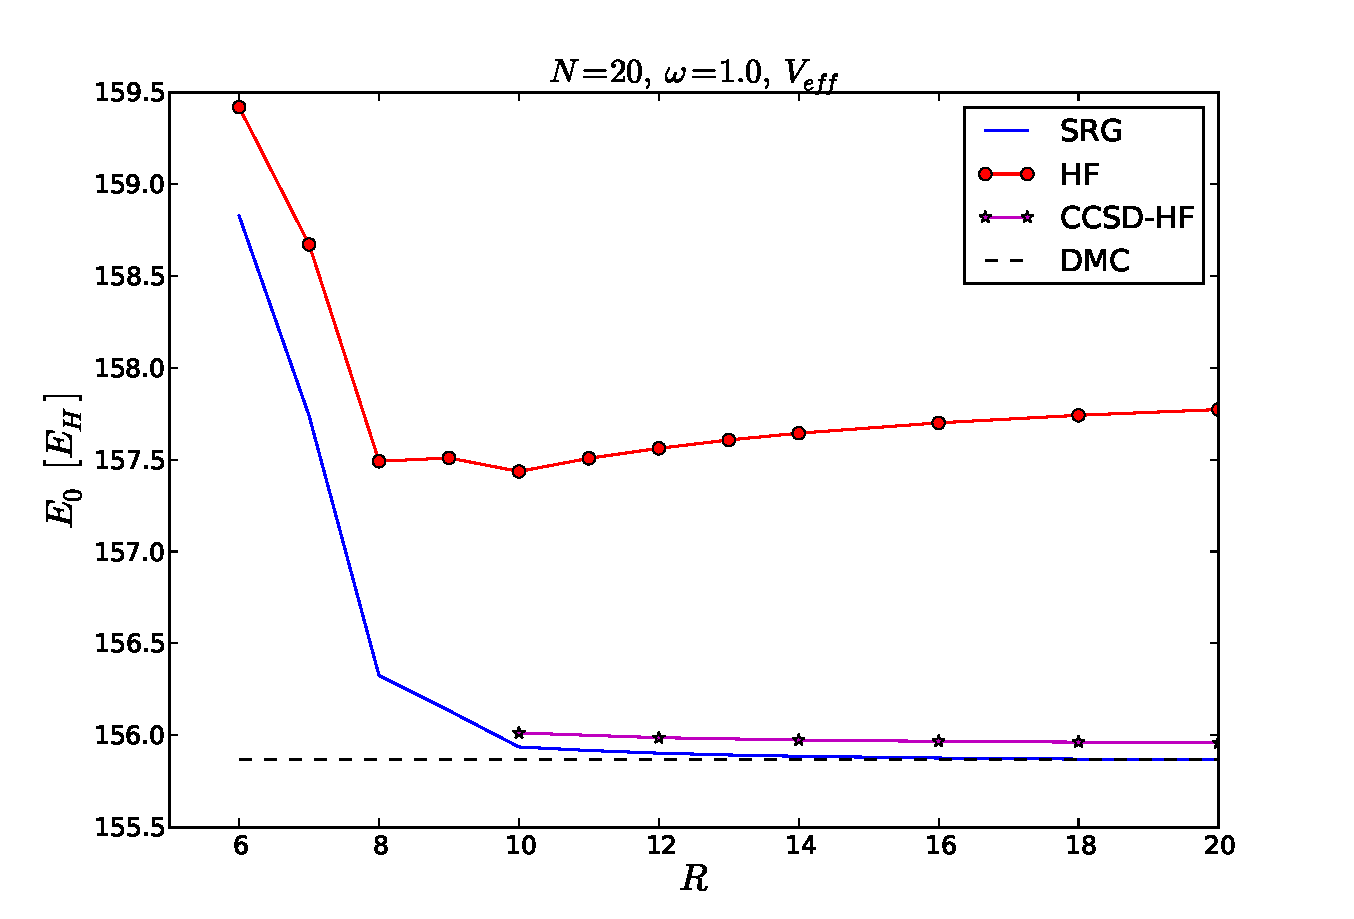
\includegraphics[scale=0.34]{../Plots/comp20parteff.pdf}}}
\mbox{\subfigure[$N=6, \omega=0.5$, Std. interaction]{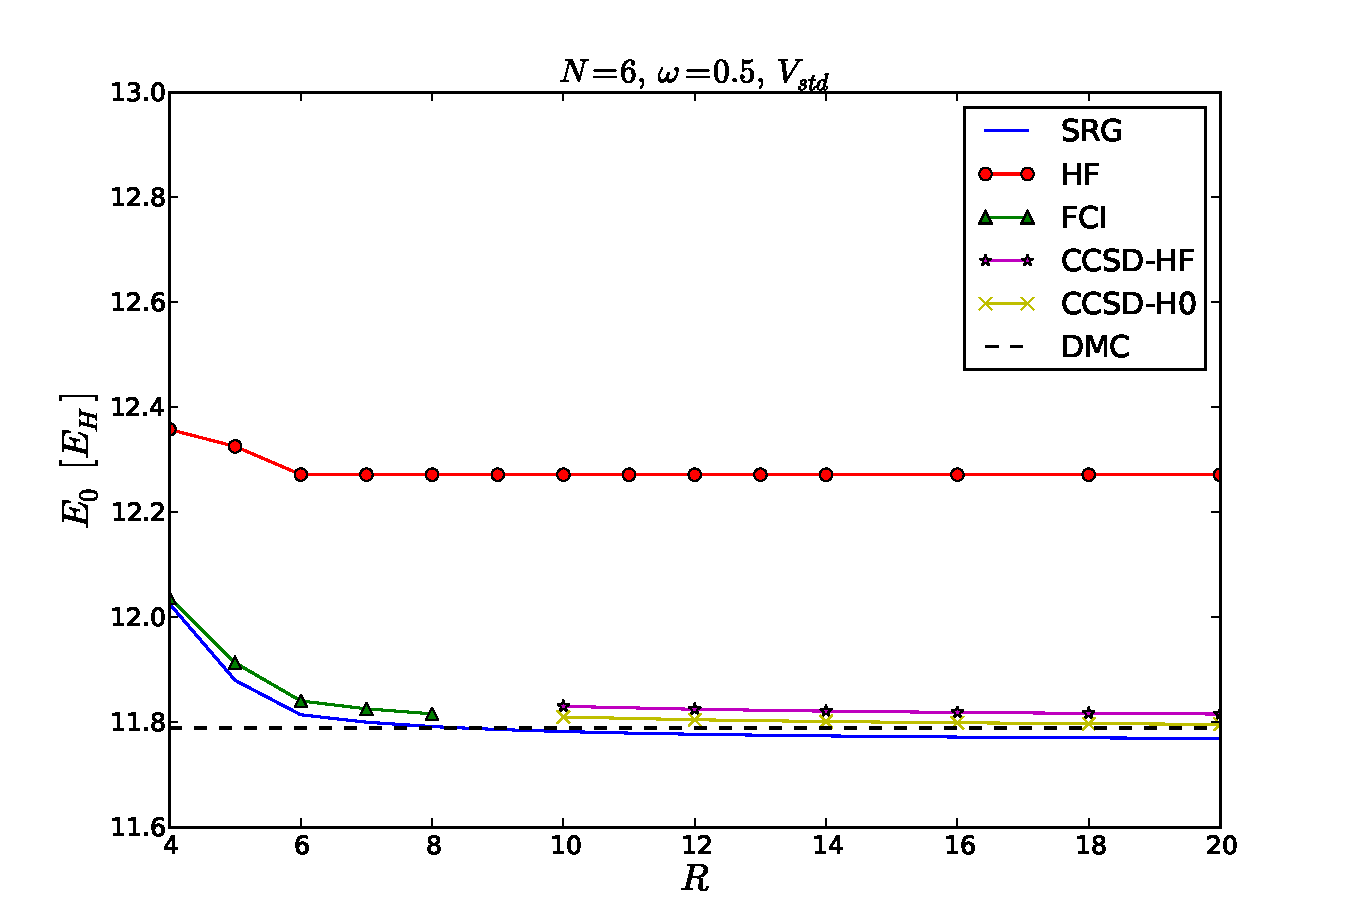
\includegraphics[scale=0.34]{../Plots/comp6partstd05.pdf}}
\subfigure[$N=6, \omega=0.5$, Eff. interaction]{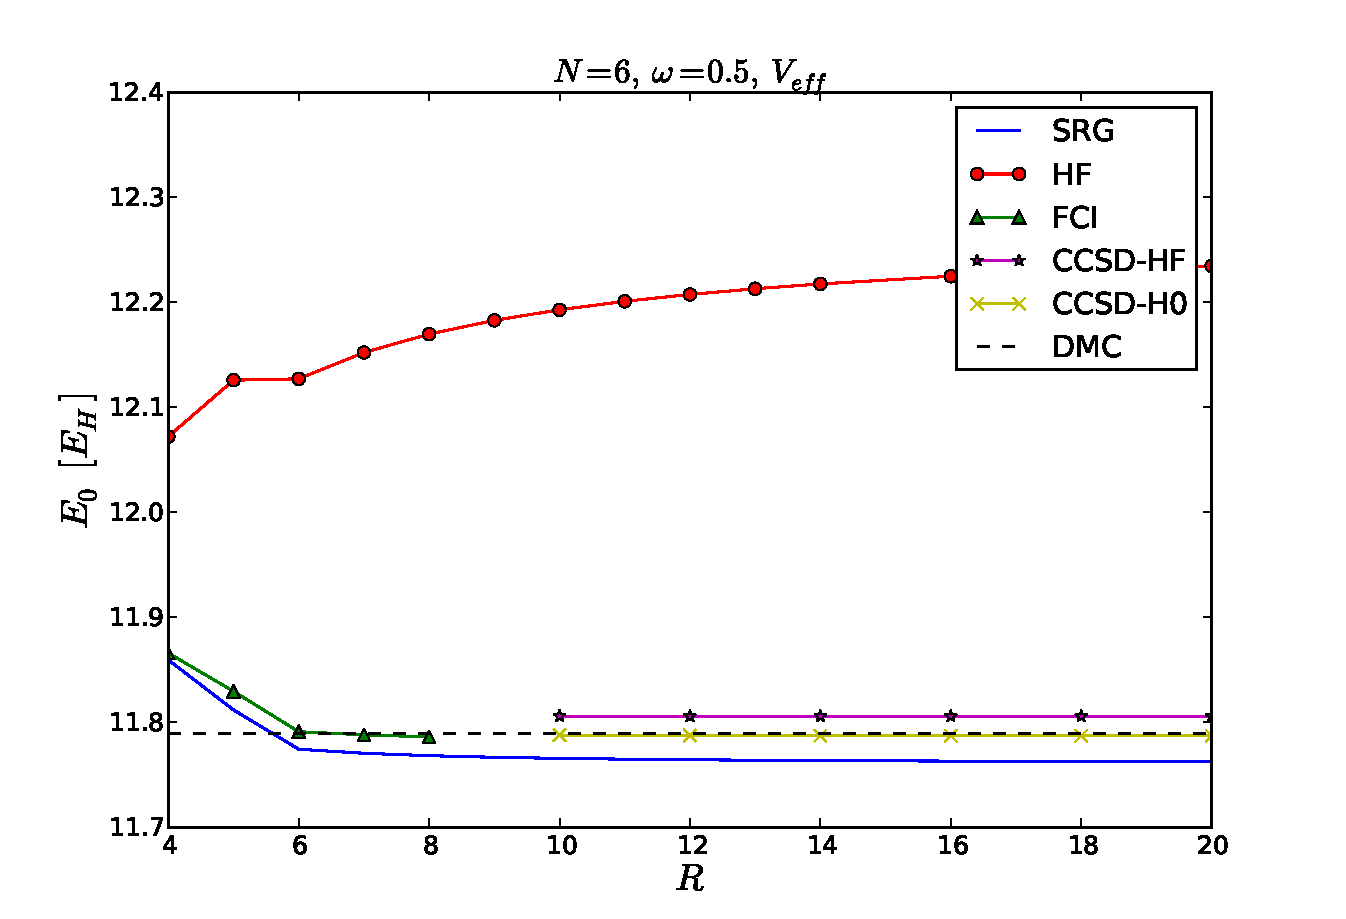
\includegraphics[scale=0.34]{../Plots/comp6parteff05.pdf}}}
\mbox{\subfigure[$N=6, \omega=0.28$, Std. interaction]{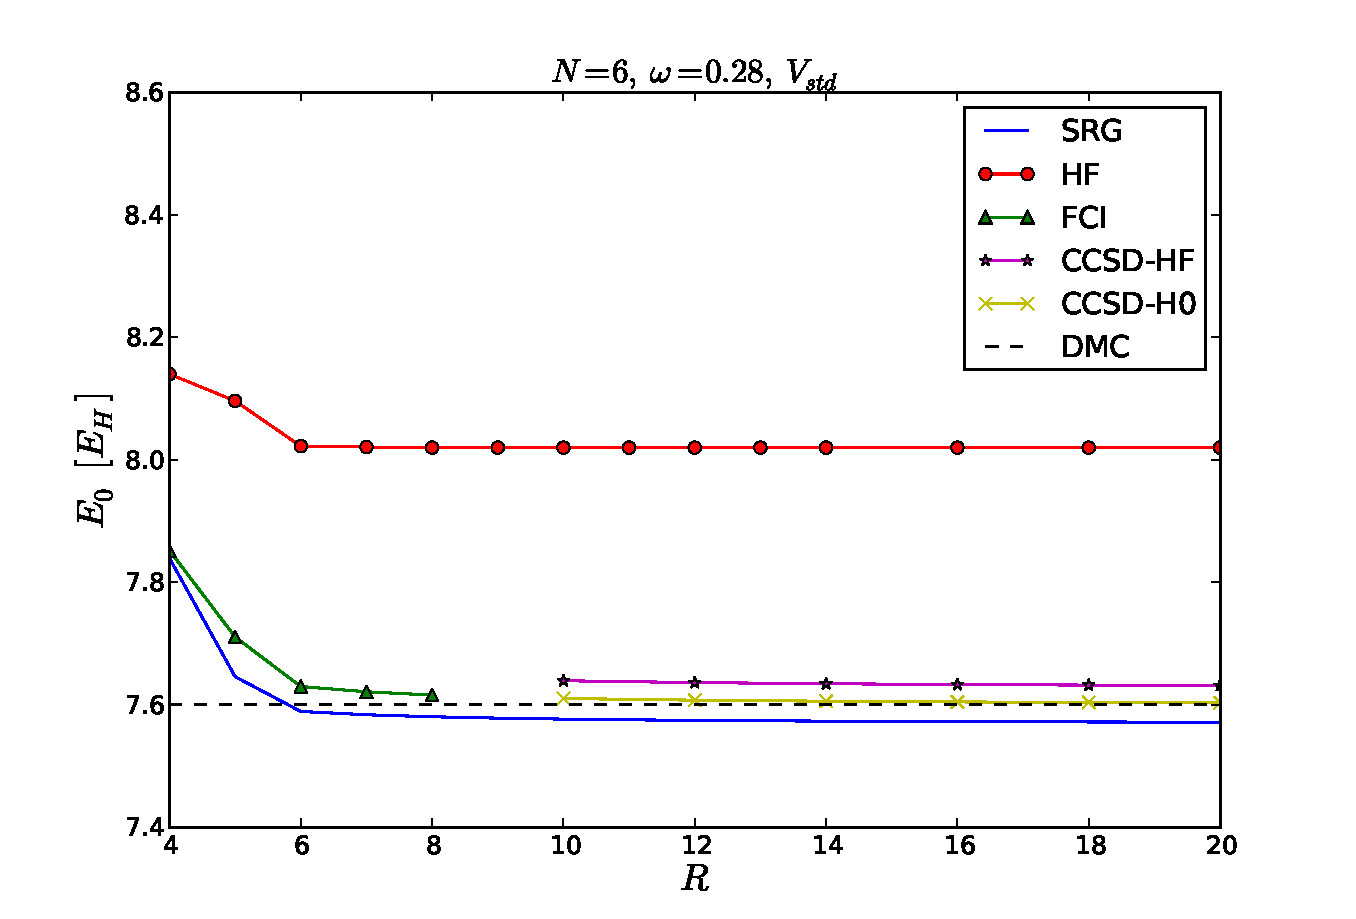
\includegraphics[scale=0.34]{../Plots/comp6partstd028.pdf}}
\subfigure[$N=6, \omega=0.28$, Eff. interaction]{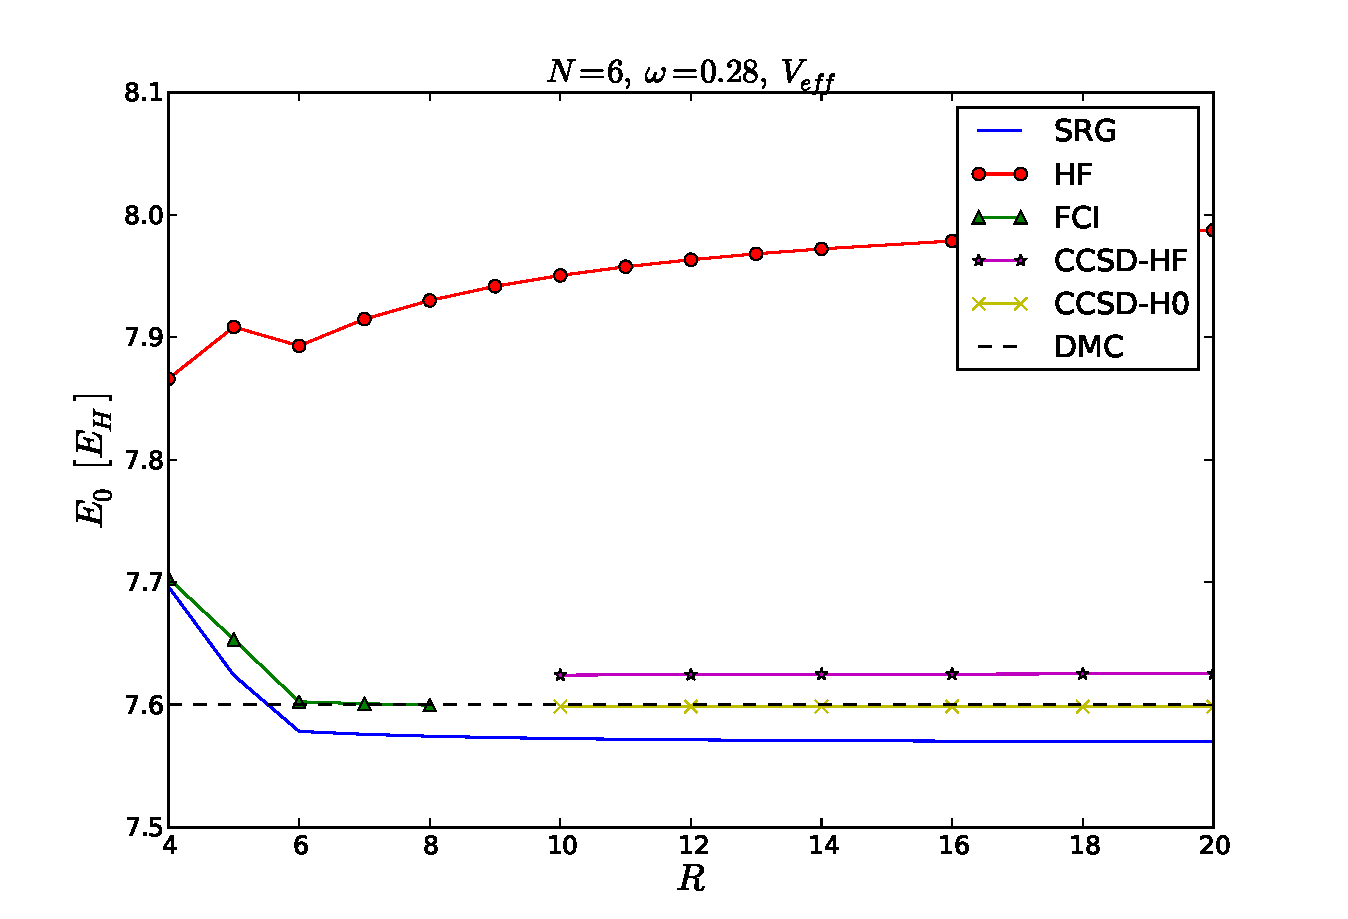
\includegraphics[scale=0.34]{../Plots/comp6parteff028.pdf}}}
\caption{Same caption as figure \ref{fig:compall0}. First we continue with $\omega=1.0$ for $N=20$ particles, then we give examples for lower values of the oscillator frequency $\omega$. For $N=20$ particles, we had not enough FCI and CCSD-HO data available to include them in the figures. }
\label{fig:compall1}
\end{center}
\end{figure}

\begin{figure}
\begin{center}
\mbox{\subfigure[$N=12, \omega=0.28$, Std. interaction]{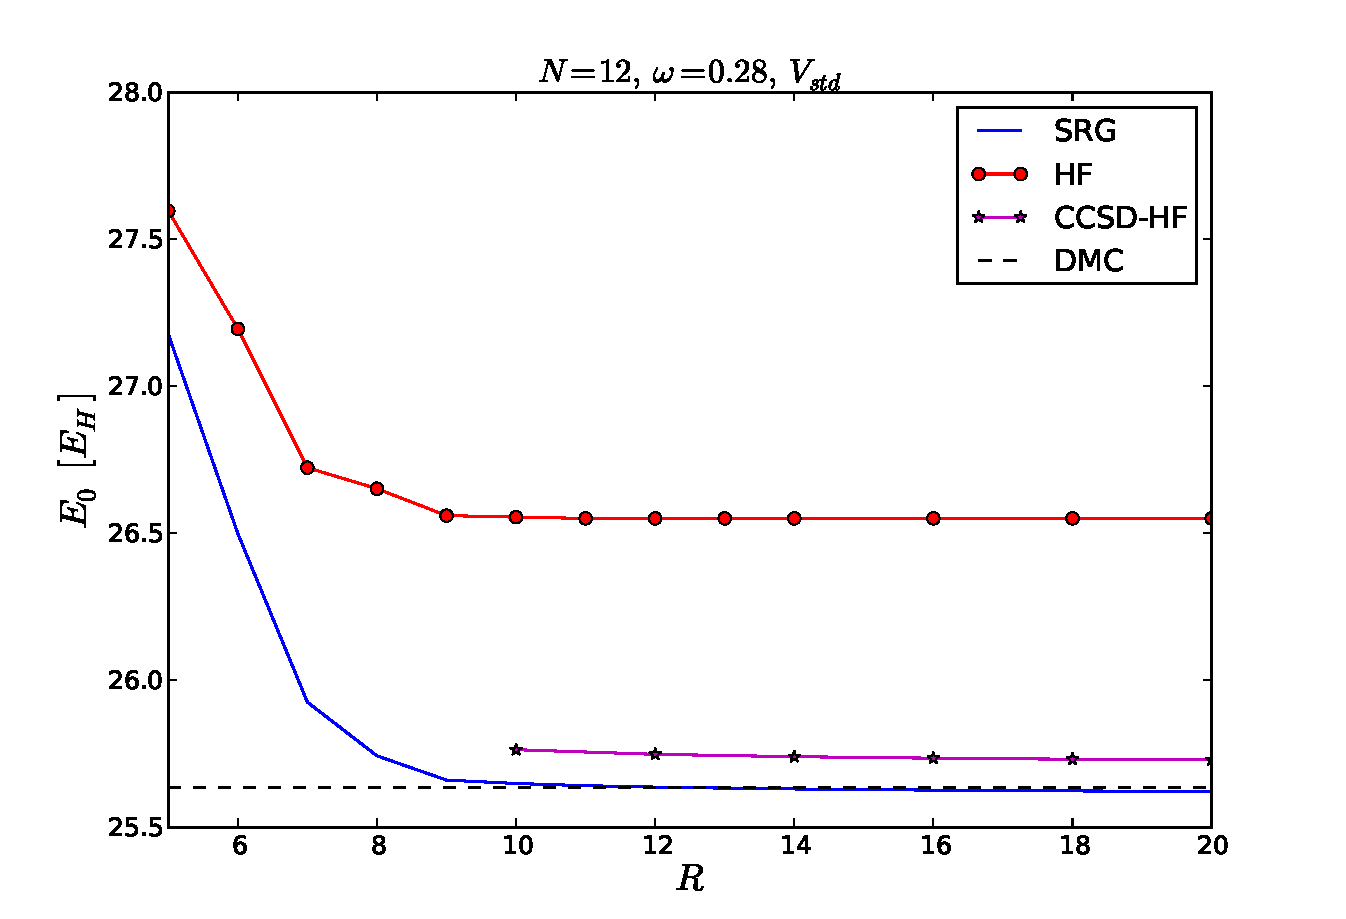
\includegraphics[scale=0.34]{../Plots/comp12partstd028.pdf}}
\subfigure[$N=12, \omega=0.28$, Eff. interaction]{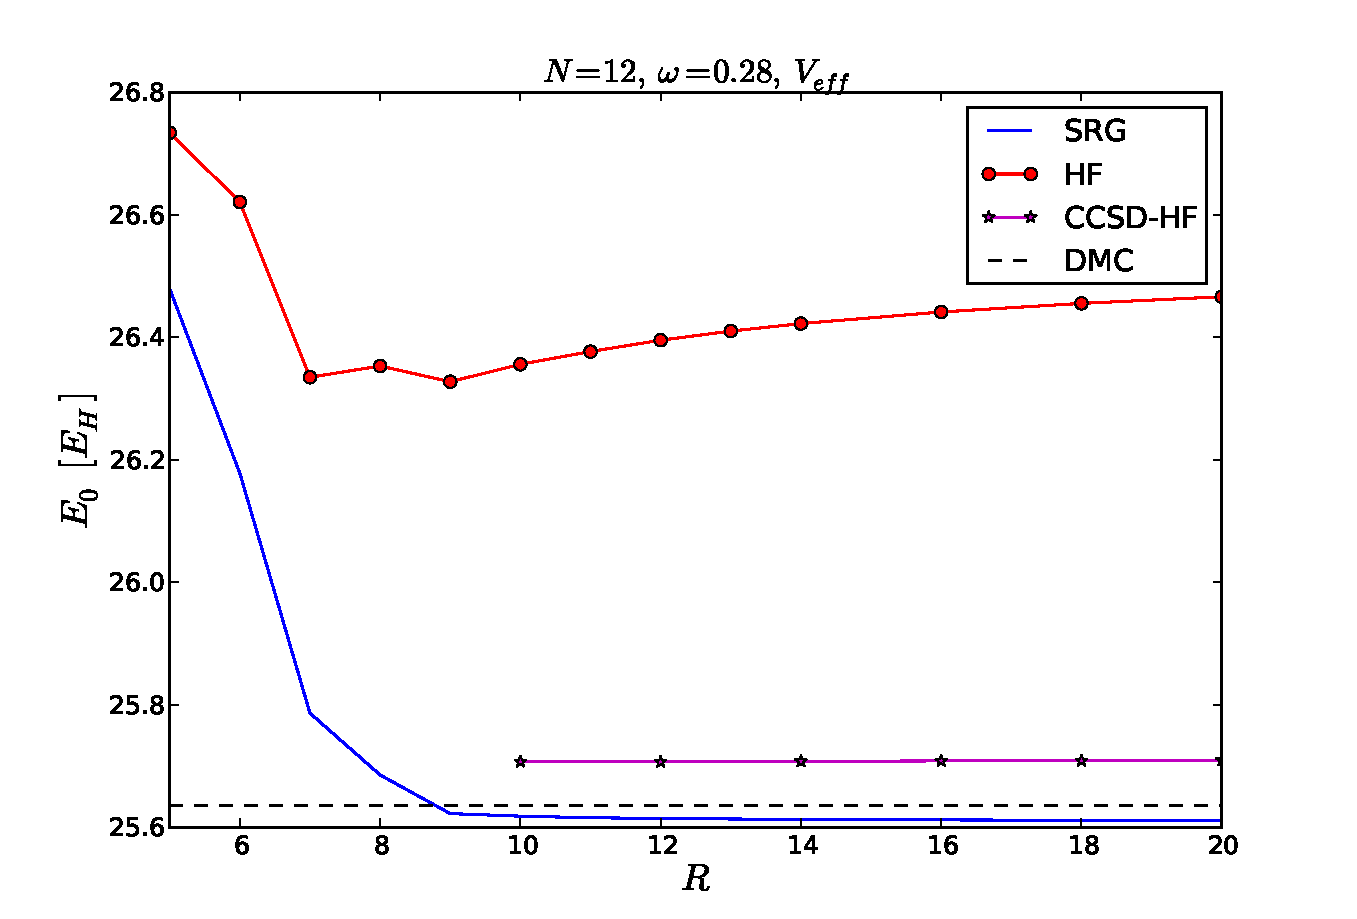
\includegraphics[scale=0.34]{../Plots/comp12parteff028.pdf}}}
\mbox{\subfigure[$N=6, \omega=0.1$, Std. interaction]{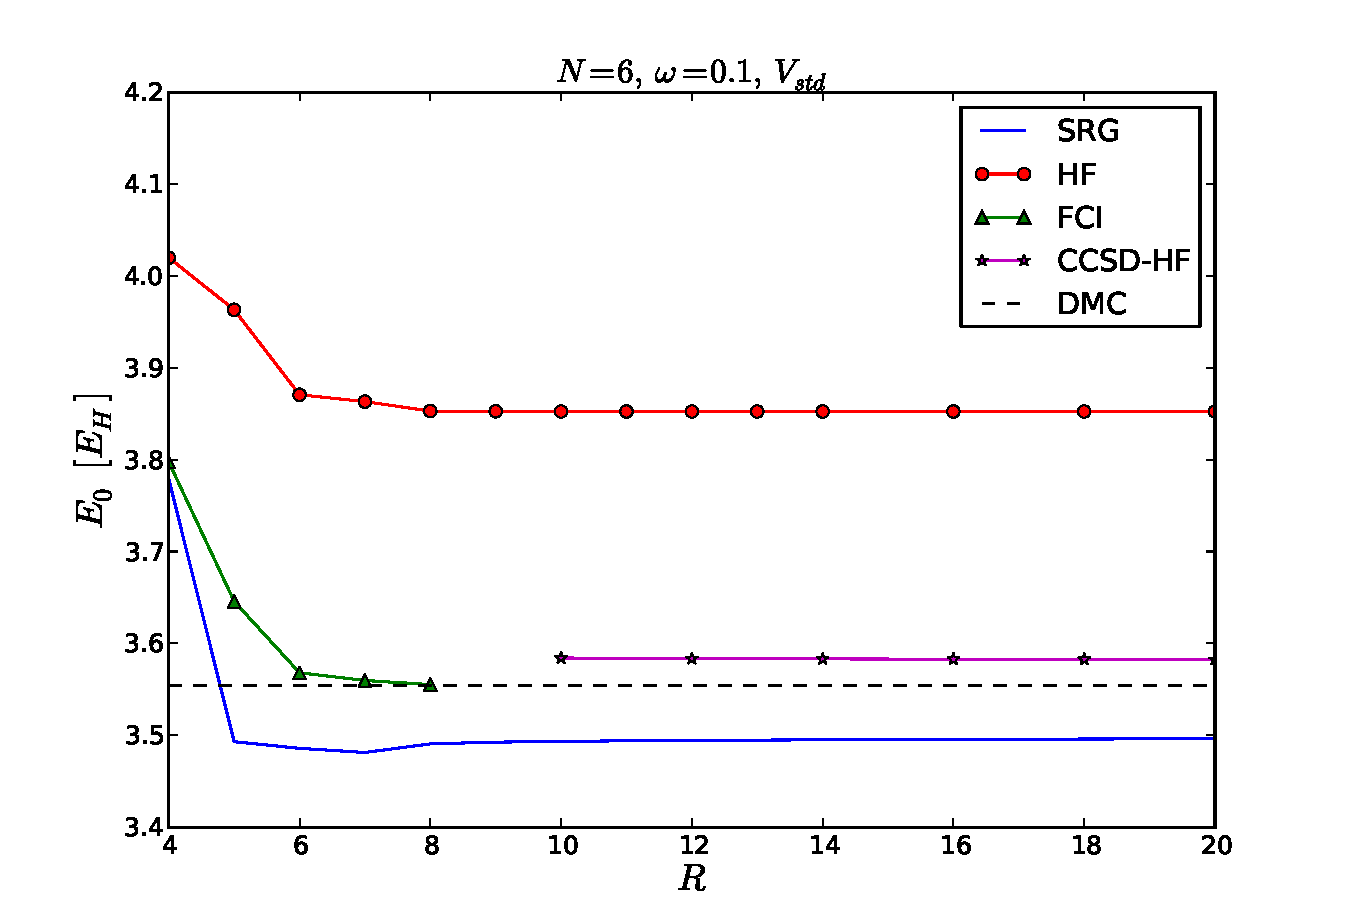
\includegraphics[scale=0.34]{../Plots/comp6partstd01.pdf}}
\subfigure[$N=6, \omega=0.1$, Eff. interaction]{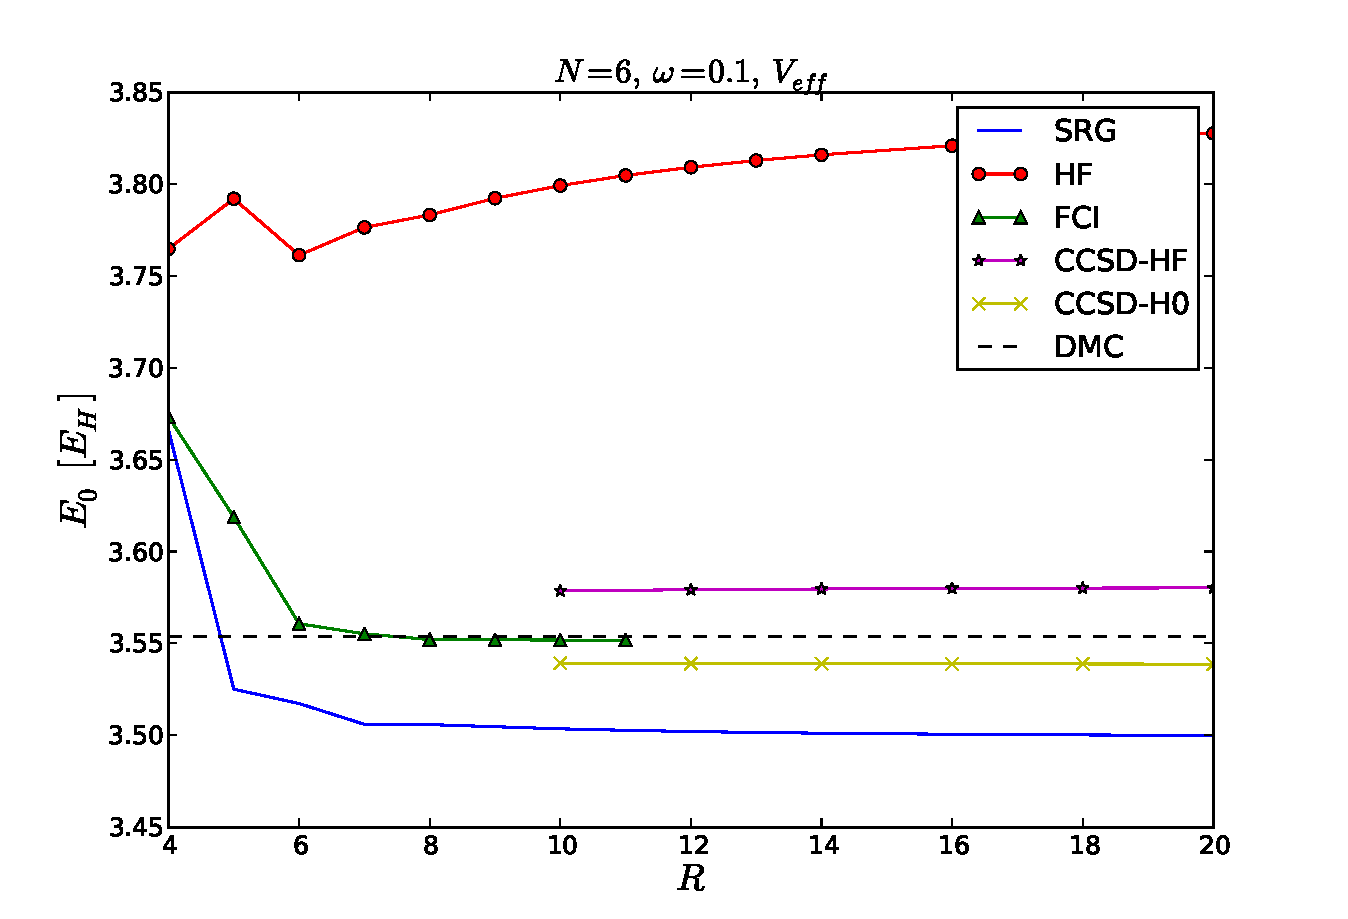
\includegraphics[scale=0.34]{../Plots/comp6parteff01.pdf}}}
\caption{Same caption as figure \ref{fig:compall0}, here examples with lower values of the oscillator frequency $\omega$. In the cases where no FCI and CCDS-HO data are included in the plots, we had not enough data available. }
\label{fig:compall2}
\end{center}
\end{figure}
